\documentclass[12pt,a4paper]{article}
\usepackage{amssymb}  %mathbb
\usepackage{amsmath}  %align
\usepackage{amsthm}   %newtheorem
\usepackage{hyperref} %a href
\usepackage{graphicx} %jpg
\usepackage[a4paper,top=1.3cm,bottom=1.3cm,left=1.3cm,right=1.3cm]{geometry}
\pagestyle{headings}
\title{Matem\'atica e Espiritualidade}
\date{}
\begin{document}
	\maketitle

	\tableofcontents
	\addtocontents{}{\protect\rule{\textwidth}{.2pt}\par}

	\section{Lista de S\'imbolos}\label{simbolos}
		\begin{flushright}
		\end{flushright}

		$ \alpha_\omega = $ Deus

		$ \infty = $ Infinito

		$ \forall \epsilon_0 = $ para todo $ \epsilon_0 $, dado $ \epsilon_0 $, \href{http://en.wikipedia.org/wiki/Universal\_quantification}{qualquer} que seja $ \epsilon_0 $

		$ \exists \delta_0 = $ \href{http://en.wikipedia.org/wiki/Existential\_quantifier}{existe} $ \delta_0 $, para algum $ \delta_0 $, para ao menos um $ \delta_0 $

		Conjunto dos n\'umeros racionais:
		\begin{align*}
			\mathbb{Q} = \left\{\frac{p}{q} ; \forall p,q \in \mathbb{Z}, q \neq 0\right\}
		\end{align*}

		Conjunto das fun\c{c}\~oes:
		\begin{align*}
			\mathbb{F}[X,Y] = \left\{f: X \rightarrow Y \, | \, \forall x \in X, \exists \, ! \, y \in Y ; f(x) = y \right\}
		\end{align*}

		Conjunto das fun\c{c}\~oes injetivas:
		\begin{align*}
			I[X,Y] = \left\{f \in \mathbb{F} : \forall a, b \in \mbox{ Im }f ; f(a) = f(b) \Rightarrow a = b \right\}
		\end{align*}

		Conjunto das fun\c{c}\~oes sobrejetivas:
		\begin{align*}
			S[X,Y] = \left\{f \in \mathbb{F} : \forall y \in Y, \exists x \in X ; f(x) = y \right\}
		\end{align*}

		Conjunto das fun\c{c}\~oes bijetivas:
		\begin{align*}
			\mathbb{B}[X,Y] = S \cap I
		\end{align*}

	\section{Quem \href{http://sites.google.com/site/mathspirituality/portugues/EuSou.ASF?attredirects=0}{sou}}
		\begin{flushright}
		\end{flushright}

		Eu sou um ser de \textquotedblleft planos\textquotedblright\, e dimens\~oes variadas: emocional\footnotemark[1], sentimental, verbal\footnotemark[1], mental\footnotemark[1] e espiritual.

		Eu sou equilibrado, proporcional, cont\'inuo [Se\c{c}\~ao \ref{continuidade}] e l\'ogico \cite{logica} (em oposi\c{c}\~ao a irracional e m\'istico. O que transcende a l\'ogica? O incomunic\'avel. O que existiu antes ou existir\'a depois dela. Mistifica\c{c}\~ao.)

		Eu sou existencial. (O ser \'e, mesmo que se recuse a ser. Se o animal n\~ao sabe o que \'e ser, j\'a o homem [Se\c{c}\~ao \ref{homem}] n\~ao sabe o que \'e n\~ao ser.)

		Eu sou $ \infty $ em possibilidades \cite{possibilidades} potenciais.

		Eu sou aut\^entico, livre, completo, espont\^aneo, simples, ben\'evolo, belo e desejante da unidade \cite{unidade} com o Todo.

		Eu sou expressivo e art\'istico.

		Eu sou progressivo, orientado \`a felicidade, perfeito [Se\c{c}\~ao \ref{serPerfeito}] num envolt\'orio eg\'oico, em aperfei\c{c}oamento \cite{aperfeicoamento}, mut\'avel, imagin\'ario, paradigm\'atico, indefinido e personalista.

		Eu sou factual, fun\c{c}\~ao de minhas experi\^encias.

		Eu sou minha atitude\footnotemark[1] diante de cada uma delas.

		Eu sou uma constante descoberta, uma busca por uma Verdade [Se\c{c}\~ao \ref{verdade}] (em cuja aproxima\c{c}\~ao tenho f\'e\cite{feh}), uma realidade dial\'etica em constru\c{c}\~ao.

		Eu sou f\'isico [Se\c{c}\~ao \ref{fisica}], din\^amico, de fun\c{c}\~ao a desempenhar, projetado para interagir com a Natureza interdimensional.

		Eu sou um ser de n\'ivel hier\'arquico e comparativo.

		Eu sou harm\^onico e em sintonia com outros seres.

		Eu sou um ser social\cite{social}, de rela\c{c}\~oes entre apar\^encias e ess\^encias [Se\c{c}\~ao \ref{essencia}].

		Logo, eu sou uma tr\'iade de fluxos: \'intimo, ilus\'orio \cite{ilusao} e exterior.

		Eu sou o que fa\c{c}o\footnotemark[1], o resultado de um trabalho. Portanto, \textbf{serei} resultado do trabalho de hoje.

		\footnotetext[1]{dualidade moral \cite{dual}} %para a secao quem sou

		\begin{flushright}
		\end{flushright}

		N\~ao sou a mat\'eria \cite{materia}, mas estou num universo relativizado \cite{relat}, composto de fluido c\'osmico universal (que forma mat\'eria e energia), regido por for\c{c}as duais \cite{dual}, agregadoras e desagregadoras, eletromagn\'eticas e espa\c{c}o-temporais \cite{tempo}.

		Num reino animal, gerado pela energia sexual.

	\section{Matem\'atica}
			\begin{flushright}
			\end{flushright}


		\subsection{\href{http://lib.org.by/_djvu/M_Mathematics/}{Livros}}
			\begin{flushright}
			\end{flushright}

			Veja tamb\'em o \href{http://www.4shared.com/dir/16354738/cea382c8/sharing.html}{\emph{4shared}} e o \href{http://sites.google.com/site/mathspirituality/}{\emph{google}}.

		\subsection{Ensino Fundamental}
			\begin{flushright}
			\end{flushright}

			Veja \cite{planetas}.

		\subsection{Superior}
			\begin{flushright}
			\end{flushright}

			Geometria Diferencial \cite{igd}

			Trajet\'oria de Avi\~ao \cite{aviao}

			Resum\~ao de \'Algebra I \cite{alg1}

			Resum\~ao de An\'alise I \cite{an1}

			A maioria \cite{metricos} das fun\c{c}\~oes \'e surreal.

			\begin{flushright}
			\end{flushright}

			\href{https://github.com/boralaemcasa/propagation/tree/master/webs%20dot%20com/math/Vinicius_Monografia.pdf}{Monografia}

			\underline{Matem\'atica Elementar} \cite{elementar}
			O Princ\'ipio da contradi\c{c}\~ao entre verdadeiro e falso.
			Definir.
			Deixar conceitos sem defini\c{c}\~ao.
			Modelar: Quais os melhores axiomas? [Se\c{c}\~ao \ref{continuidade}]
			Consequ\^encias.

			\begin{flushright}
			\end{flushright}

			Os Axiomas \cite{euclides} de Euclides [Se\c{c}\~ao \ref{escAxiomas}]

			\'Algebra Linear I \cite{linear1}

			Geometria Espacial \cite{espacial}

			\begin{flushright}
			\end{flushright}

			Geometria Inversiva \cite{inversiva}

			Equa\c{c}\~oes C\'ubicas \cite{cubicas}

			Equa\c{c}\~oes Diofantinas \cite{diofantinas}

			$ \pi $ e Fra\c{c}\~oes Cont\'inuas \cite{fracoes}

			Quat\'ernions \cite{Quaternions}

			Oct\'onions \cite{octonions}

			Probabilidade de o universo ter sido criado por \href{http://www.creationofuniverse.com/html/equilibrium03.html}{coincid\^encia}.

			\subsubsection{Continuidade}\label{continuidade}
			\begin{flushright}
			\end{flushright}

				\newtheoremstyle{meuEstilo}{}{}{}{}{\bfseries}{:}{ }{#1}
				\theoremstyle{meuEstilo}

				\newtheorem{Q1}{Quest\~ao 1}
				\begin{Q1} Na natureza, qual cardinalidade tende a zero?
				\end{Q1}

				Talvez a resposta esteja no tempo \cite{tempo} de maia-vida.

				A redu\c{c}\~ao do universo cont\'inuo ao universo de Planck [Se\c{c}\~ao \ref{fisica}] \'e id\^entica \`a restri\c{c}\~ao de $ \mathbb{R} $ a $ \mathbb{Q} $.

				De acordo com os estudos de \href{http://en.wikipedia.org/wiki/Cardinality_of_the_continuum}{Cantor}, todos os enumer\'aveis podem ser colocados em correspond\^encia biun\'ivoca.
				Podemos come\c{c}ar de um e chegar ao en\'esimo. Indu\c{c}\~ao matem\'atica.

				Seja, ent\~ao, para cada objeto, um n\'umero e para cada n\'umero um ponto.

				Vamos agora trabalhar com conjuntos abertos e fechados. Pois $(a, \infty)$ pode ser bijetivado com $(b, c)$ e $[a,b]$ com $[c,d]$.

			\subsubsection{$ \infty $ e Cardinalidades}
			\begin{flushright}
			\end{flushright}

				Tem propriedades do zero: $ \infty + \infty = \infty = (a + bi) \cdot \infty $

				Tem propriedades da unidade: $ \infty \cdot \infty = \infty = \infty ^ \infty $

				O oposto pode n\~ao ser alg\'ebrico: $ \infty + (- \infty )$ pode ser igual a zero, menor ou maior que $0$.

				\begin{align*}
					\underset{x \rightarrow \infty}{\operatorname{\lim}} f(x) = L \\
					\underset{x \rightarrow a}{\operatorname{\lim}} g(x) = \infty \\
					\underset{x \rightarrow \infty}{\operatorname{\lim}} h(x) = \infty \\
					0 \cdot \infty, 1^ \infty, 0^0, \frac{0}{0}, \frac{\infty}{\infty}...
				\end{align*}

				\emph{isso vai longe!...}

				$ \infty $ \'e o lugar geom\'etrico onde se encontram retas parelelas em uma certa dire\c{c}\~ao.

				Logo, $f'(x) = g'(x)$ quando $ x \rightarrow \infty \Rightarrow f, g $ se tocam no mesmo ponto no $ \infty $.

		\subsection{Hist\'oria | Correntes de Pensamento}
			\begin{flushright}
			\end{flushright}

			\textbf{-VII/-VI}

			\href{http://pt.wikipedia.org/wiki/Tales_de_Mileto}{Tales} de Mileto (624-546 a.C.) | Geometria em $ \mathbb{R}^2 $

			\begin{flushright}
			\end{flushright}

			\textbf{-VI/-V}

			\href{http://en.wikipedia.org/wiki/Pythagoras}{Pit\'agoras} de Samos (570-495 a.C.) | Geometria em $ \mathbb{R}^2 $

			\begin{flushright}
			\end{flushright}

			\textbf{-IV}

			\href{http://en.wikipedia.org/wiki/Menaechmus}{Menaechmus} of Alopeconnesus (380-320 a.C.) | Geometria em $ \mathbb{R}^3 $

			\begin{flushright}
			\end{flushright}

			\textbf{-IV/-III}

			\href{http://pt.wikipedia.org/wiki/Euclides}{Euclides} de Alexandria (360-265 a.C.) | Geometria em $ \mathbb{R}^2 $, Aritm\'etica

			\begin{flushright}
			\end{flushright}

			\textbf{-III}

			\href{http://en.wikipedia.org/wiki/Archimedes#Mathematics}{Archimedes} of Syracuse (287-212 a.C.) | C\'alculo

			\begin{flushright}
			\end{flushright}

			\textbf{-III/-II}

			\href{http://pt.wikipedia.org/wiki/Erat\%C3\%B3stenes}{Erat\'ostenes} (276-195 a.C.) | \'Algebra. Poeta, atleta e ge\'ografo.

			\begin{flushright}
			\end{flushright}

			\textbf{-II/-I}

			\href{http://en.wikipedia.org/wiki/Posidonius}{Posidonius} of Apameia / Rhodes (135-51 a.C.) | Geometria Projetiva. Pol\'imata.

			\begin{flushright}
			\end{flushright}

			\textbf{I}

			\href{http://pt.wikipedia.org/wiki/Heron_de_Alexandria}{Her\~ao}  / Heron / Hero de Alexandria (10-70) | Geometria em $ \mathbb{R}^2 $

			\begin{flushright}
			\end{flushright}

			\textbf{I-II}

			\href{http://en.wikipedia.org/wiki/Nicomachus}{Nicomachus} of Gerasa (60-120) | Aritm\'etica. Pitag\'orico.

			\href{http://pt.wikipedia.org/wiki/Menelau_de_Alexandria}{Menelau} de Alexandria (70-140) | Geometria em $ \mathbb{R}^3 $

			\begin{flushright}
			\end{flushright}

			\textbf{III}

			\href{http://pt.wikipedia.org/wiki/Diofanto_de_Alexandria}{Diofanto} de Alexandria (200-98) | \'Algebra

			\begin{flushright}
			\end{flushright}

			\textbf{III-IV}

			\href{http://en.wikipedia.org/wiki/Pappus_of_Alexandria}{Pappus} de Alexandria (290-350) | Geometria Projetiva

			\href{http://en.wikipedia.org/wiki/Sun_Tzu_(mathematician)}{Sun Tzu} / Sun Zi (301?-600?) | \'Algebra

			\begin{flushright}
			\end{flushright}

			\textbf{XI}

			\href{http://en.wikipedia.org/wiki/Yusuf_al-Mu\%27taman_ibn_Hud}{Hud}, Yusuf ibn Ahmad al-Mu'taman ibn Hud (10xx) | Geometria em $ \mathbb{R}^2 $

			\begin{flushright}
			\end{flushright}

			\textbf{XII}

			\href{http://pt.wikipedia.org/wiki/Bhaskara}{Bhaskara} (1114-85) | Equa\c{c}\~oes de segundo grau

			\begin{flushright}
			\end{flushright}

			\textbf{XII-XIII}

			\href{http://pt.wikipedia.org/wiki/Leonardo_Fibonacci}{Fibonacci}, Leonardo (1170-1250) | Teoria de N\'umeros

			\begin{flushright}
			\end{flushright}

			\textbf{XIII}

			\href{http://en.wikipedia.org/wiki/Qin_Jiushao}{Jiushao}, Qin (1202-61) | \'Algebra

			\begin{flushright}
			\end{flushright}

			\textbf{XV-XVI}

			\href{http://en.wikipedia.org/wiki/Luca_Pacioli}{Pacioli}, Luca Bartolomeo de (1446-1517) | Financeira. Franciscano.

			\begin{flushright}
			\end{flushright}

			\textbf{XVI}

			\href{http://pt.wikipedia.org/wiki/Girolamo_Cardano}{Cardano}, Gerolamo (1501-76) | Equa\c{c}\~oes de terceiro e quarto grau. Pol\'imata na jogatina!

			\begin{flushright}
			\end{flushright}

			\textbf{XVI-XVII}

			\href{http://pt.wikipedia.org/wiki/John_Napier}{Napier}, John (1550-1617) | Logaritmos

			\href{http://en.wikipedia.org/wiki/Johannes_Kepler}{Kepler}, Johannes (1571-1630) | Geometria em $ \mathbb{R}^3 $

			\href{http://pt.wikipedia.org/wiki/Marin_Mersenne}{Mersenne}, Marin / le Père (1588-1648) | \'Algebra. M\'usico te\'orico.

			\href{http://en.wikipedia.org/wiki/Desargues}{Desargues}, G\'erard (1591-1661) | Geometria Projetiva

			\href{http://en.wikipedia.org/wiki/Albert_Girard}{Girard}, Albert (1595-1632) | \'Algebra

			\href{http://pt.wikipedia.org/wiki/Ren\%C3\%A9_Descartes}{Descartes}, Ren\'e (1596-1650) | Geometria Anal\'itica

			\begin{flushright}
			\end{flushright}

			\textbf{XVII}

			\href{http://pt.wikipedia.org/wiki/Pierre_de_Fermat}{Fermat}, Pierre de (1601-65) | Teoria de N\'umeros. Advogado...

			\href{http://en.wikipedia.org/wiki/John_Pell}{Pell}, John (1611-85) | \'Algebra

			\href{http://pt.wikipedia.org/wiki/Blaise_Pascal}{Pascal}, Blaise (1623-62) | Combinat\'oria. Fil\'osofo da religi\~ao...

			\begin{flushright}
			\end{flushright}

			\textbf{XVII-XVIII}

			\href{http://pt.wikipedia.org/wiki/Isaac_Newton}{Newton}, Isaac (1643-1727) | C\'alculo. Te\'ologo alquimista!

			\href{http://pt.wikipedia.org/wiki/Gottfried_Leibniz}{Leibniz}, Gottfried Wilhelm (1646-1716) | C\'alculo. Pol\'imata.

			\href{http://en.wikipedia.org/wiki/Giovanni_Ceva}{Ceva}, Giovanni (1647-1734) | Geometria em $ \mathbb{R}^2 $

			\href{http://en.wikipedia.org/wiki/Michel_Rolle}{Rolle}, Michel (1652-1719) | An\'alise

			\href{http://pt.wikipedia.org/wiki/Jakob_Bernoulli}{Bernoulli}, Jacob / James / Jacques (1654-1705) | Equa\c{c}\~oes Diferenciais. Te\'ologo...

			\href{http://pt.wikipedia.org/wiki/Guillaume_Fran\%C3\%A7ois_Antoine,_Marqu\%C3\%AAs_de_l\%27H\%C3\%B4pital}{l'H\^opital}, Guillaume Fran\c{c}ois Antoine, Marquis de (1661-1704) | An\'alise

			\href{http://en.wikipedia.org/wiki/Saccheri}{Saccheri}, Giovanni Girolamo (1667-1733) | Geometria Hiperb\'olica. Padre jesu\'ita...

			\href{http://en.wikipedia.org/wiki/Demoivre}{de Moivre}, Abraham (1667-1754) | An\'alise Complexa

			\href{http://en.wikipedia.org/wiki/Ricatti}{Ricatti}, Jacopo Francesco (1676-1754) | Equa\c{c}\~oes Diferenciais

			\href{http://pt.wikipedia.org/wiki/Brook_Taylor}{Taylor}, Brook (1685-1731) | An\'alise

			\href{http://en.wikipedia.org/wiki/Christian_Goldbach}{Goldbach}, Christian (1690-1764) | Teoria de N\'umeros

			\href{http://en.wikipedia.org/wiki/Colin_Maclaurin}{Maclaurin}, Caulin (1698-1746) | An\'alise

			\begin{flushright}
			\end{flushright}

			\textbf{XVIII}

			\href{http://pt.wikipedia.org/wiki/Daniel_Bernoulli}{Bernoulli}, Daniel (1700-82) | Equa\c{c}\~oes Diferenciais

			\href{http://en.wikipedia.org/wiki/Gabriel_Cramer}{Cramer}, Gabriel (1704-52) | \'Algebra Linear

			\href{http://pt.wikipedia.org/wiki/Leonhard_Euler}{Euler}, Leonhard (1707-83) | An\'alise Complexa. Inerrante b\'iblico...

			\href{http://pt.wikipedia.org/wiki/Alembert}{d'Alembert}, Jean le Rond (1717-83) | An\'alise

			\href{http://en.wikipedia.org/wiki/Johann_Heinrich_Lambert}{Lambert}, Johann Heinrich (1728-77) | Geometria Hiperb\'olica, Equa\c{c}\~oes Diferenciais

			\href{http://en.wikipedia.org/wiki/John_Wilson_(mathematician)}{Wilson}, John (1741-93) | \'Algebra

			\begin{flushright}
			\end{flushright}

			\textbf{XVIII-XIX}

			\href{http://pt.wikipedia.org/wiki/Lagrange}{Lagrange}, Joseph-Louis (1736-1813) | An\'alise

			\href{http://en.wikipedia.org/wiki/Gaspard_Monge}{Monge}, Gaspard (1746-1818) | Geometria Descritiva

			\href{http://pt.wikipedia.org/wiki/Pierre_Simon_Laplace}{Laplace}, Pierre-Simon (1749-1827) | Equa\c{c}\~oes Diferenciais, \'Algebra Linear

			\href{http://en.wikipedia.org/wiki/Lhuilier}{L'Huilier}, Simon Antoine Jean (1750-1840) | An\'alise

			\href{http://pt.wikipedia.org/wiki/Adrien-Marie_Legendre}{Legendre}, Adrien-Marie (1752-1833) | An\'alise

			\href{http://pt.wikipedia.org/wiki/Marc-Antoine_Parseval}{Parseval}, Marc-Antoine (1755-1836) | Equa\c{c}\~oes Diferenciais. Opositor \`a revolu\c{c}\~ao francesa...

			\href{http://en.wikipedia.org/wiki/Paolo_Ruffini}{Ruffini}, Paolo (1765-1822) | \'Algebra

			\href{http://en.wikipedia.org/wiki/Jean-Robert_Argand}{Argand}, Jean-Robert (1768-1822) | An\'alise Complexa

			\href{http://pt.wikipedia.org/wiki/Jean-Baptiste_Joseph_Fourier}{Fourier}, Joseph (1768-1830) | An\'alise

			\href{http://pt.wikipedia.org/wiki/Carl_Friedrich_Gauss}{Gauss}, Carl Friedrich (1777-1855) | An\'alise Complexa

			\href{http://en.wikipedia.org/wiki/J\%C3\%B3zef_Maria_Hoene-Wro\%C5\%84ski}{Wronski}, J\'ozef Maria Hoëne (1778-1853) | Equa\c{c}\~oes Diferenciais

			\href{http://en.wikipedia.org/wiki/Poisson}{Poisson}, Sim\'eon Denis (1781-1840) | Equa\c{c}\~oes Diferenciais

			\href{http://pt.wikipedia.org/wiki/Bernard_Bolzano}{Bolzano}, Bernard (1781-1848) | An\'alise. Padre...

			\href{http://en.wikipedia.org/wiki/Charles_Julien_Brianchon}{Brianchon}, Charles Julien (1783-1864) | Geometria Projetiva

			\href{http://pt.wikipedia.org/wiki/Friedrich_Wilhelm_Bessel}{Bessel}, Friedrich (1784-1846) | Equa\c{c}\~oes Diferenciais

			\href{http://en.wikipedia.org/wiki/Jean-Victor_Poncelet}{Poncelet}, Jean-Victor (1788-1867) | Geometria Projetiva

			\href{http://pt.wikipedia.org/wiki/Augustin_Louis_Cauchy}{Cauchy}, Augustin Louis (1789-1857) | An\'alise Complexa. Jesu\'ita...

			\href{http://pt.wikipedia.org/wiki/August_Ferdinand_M\%C3\%B6bius}{Möbius}, August Ferdinand (1790-1868) | Geometria Diferencial, Projetiva

			\href{http://pt.wikipedia.org/wiki/Nikolai_Ivanovich_Lobachevsky}{Lobachevsky}, Nikolai Ivanovich (1792-1856) | Geometria Hiperb\'olica

			\href{http://pt.wikipedia.org/wiki/George_Green}{Green}, George (1793-1841) | An\'alise

			\href{http://en.wikipedia.org/wiki/Olinde_Rodrigues}{Rodrigues}, Benjamin Olinde (1795-1851) | Geometria Diferencial

			\href{http://pt.wikipedia.org/wiki/Gabriel_Lam\%C3\%A9}{Lam\'e}, Gabriel (1795-1870) | \'Algebra

			\href{http://en.wikipedia.org/wiki/Jakob_Steiner}{Steiner}, Jakob (1796-1863) | Geometria Projetiva

			\href{http://en.wikipedia.org/wiki/Von_Staudt}{von Staudt}, Karl Georg Christian (1798-1867) | Geometria Projetiva

			\href{http://en.wikipedia.org/wiki/Heinrich_Scherk}{Scherk}, Heinrich Ferdinand (1798-1885) | Geometria Diferencial

			\href{http://en.wikipedia.org/wiki/Karl_Wilhelm_Feuerbach}{Feuerbach}, Karl Wilhelm (1800-34) | Geometria em $ \mathbb{R}^2 $

			\href{http://en.wikipedia.org/wiki/Gaspare_Mainardi}{Mainardi}, Gaspare (1800-79) | Geometria Diferencial

			\begin{flushright}
			\end{flushright}

			\textbf{XIX}

			\href{http://pt.wikipedia.org/wiki/Niels_Henrik_Abel}{Abel}, Niels Henrik (1802-29) | Teoria de N\'umeros, Grupos

			\href{http://pt.wikipedia.org/wiki/J\%C3\%A1nos_Bolyai}{Bolyai}, J\'anos (1802-60) | Geometria Hiperb\'olica

			\href{http://en.wikipedia.org/wiki/Jacques_Charles_Fran\%C3\%A7ois_Sturm}{Sturm}, Jacques Charles Fran\c{c}ois (1803-55) | Equa\c{c}\~oes Diferenciais

			\href{http://pt.wikipedia.org/wiki/Carl_Gustav_Jakob_Jacobi}{Jacobi}, Carl Gustav Jacob (1804-51) | \'Algebra Linear, Teoria de N\'umeros

			\href{http://en.wikipedia.org/wiki/George_Jerrard}{Jerrard}, George Birch (1804-63) | \'Algebra

			\href{http://pt.wikipedia.org/wiki/Dirichlet}{Dirichlet}, Johann Peter Gustav Lejeune (1805-59) | An\'alise

			\href{http://pt.wikipedia.org/wiki/William_Rowan_Hamilton}{Hamilton}, William Rowan (1805-65) | \'Algebra n\~ao comutativa = Quat\'ernions

			\href{http://en.wikipedia.org/wiki/Hermann_Grassmann}{Grassmann}, Hermann Günther (1809-77) | \'Algebra Linear

			\href{http://en.wikipedia.org/wiki/Liouville}{Liouville}, Joseph (1809-82) | An\'alise Complexa, Equa\c{c}\~oes Diferenciais.

			\href{http://en.wikipedia.org/wiki/Ernst_Kummer}{Kummer}, Ernst (1810-93) | \'Algebra

			\href{http://pt.wikipedia.org/wiki/\'Evariste_Galois}{Galois}, \'Evariste (1811-32) | Teoria de N\'umeros. Anti-mon\'arquico suicida.

			\href{http://en.wikipedia.org/wiki/Pierre_Alphonse_Laurent}{Laurent}, Pierre Alphonse (1813-54) | An\'alise Complexa

			\href{http://pt.wikipedia.org/wiki/George_Boole}{Boole}, George (1815-64) | L\'ogica

			\href{http://pt.wikipedia.org/wiki/Karl_Weierstrass}{Weierstrass}, Karl (1815-97) | An\'alise

			\href{http://en.wikipedia.org/wiki/Jean_Fr\%C3\%A9d\%C3\%A9ric_Frenet}{Frenet}, Jean Fr\'ed\'eric (1816-1900) | C\'alculo Vetorial

			\href{http://en.wikipedia.org/wiki/Joseph_Alfred_Serret}{Serret}, Joseph Alfred (1819-85) | C\'alculo Vetorial

			\href{http://en.wikipedia.org/wiki/Eduard_Heine}{Heine}, Heinrich Eduard (1821-81) | An\'alise

			\href{http://en.wikipedia.org/wiki/Chebyshev_function}{Chebyshev}, Pafnuty Lvovich (1821-94) | Teoria de N\'umeros

			\href{http://en.wikipedia.org/wiki/Ferdinand_Eisenstein}{Eisenstein}, Ferdinand Gotthold Max (1823-52) | \'Algebra

			\href{http://en.wikipedia.org/wiki/Kronecker}{Kronecker}, Leopold (1823-91) | Teoria de N\'umeros. Qu\'inticas.

			\href{http://en.wikipedia.org/wiki/Delfino_Codazzi}{Codazzi}, Delfino (1824-73) | Geometria Diferencial

			\href{http://pt.wikipedia.org/wiki/Bernhard_Riemann}{Riemann}, Bernhard (1826-66) | An\'alise, Geometria, Teoria de N\'umeros. Tentou jogar matem\'atica no livro do G\^enesis

			\href{http://en.wikipedia.org/wiki/Christoffel}{Christoffel}, Elwin Bruno (1829-1900) | Geometria Diferencial

			\href{http://en.wikipedia.org/wiki/Alfred_Enneper}{Enneper}, Alfred (1830-85) | Geometria Diferencial

			\href{http://pt.wikipedia.org/wiki/Paul_du_Bois-Reymond}{du Bois-Reymond}, Paul (1831-89) | Equa\c{c}\~oes Diferenciais

			\href{http://en.wikipedia.org/wiki/Laguerre}{Laguerre}, Edmond Nicolas (1834-86) | \'Algebra Linear

			\href{http://en.wikipedia.org/wiki/Hankel}{Hankel}, Hermann (1839-73) | Equa\c{c}\~oes Diferenciais

			\href{http://en.wikipedia.org/wiki/Sophus_Lie}{Lie}, Marius Sophus (1842-99) | Grupos, Geometria e Equa\c{c}\~oes Diferenciais

			\href{http://en.wikipedia.org/wiki/Giulio_Ascoli}{Ascoli}, Giulio (1843-96) | An\'alise

			\href{http://en.wikipedia.org/wiki/William_Kingdon_Clifford}{Clifford}, William Kingdon (1845-79) | \'Algebra

			\href{http://pt.wikipedia.org/wiki/Cesare_Arzel\%C3\%A0}{Arzel\`a}, Cesare (1847-1912) | An\'alise

			\href{http://en.wikipedia.org/wiki/Carl_Gustav_Axel_Harnack}{Harnack}, Carl Gustav Axel (1851-88) | Equa\c{c}\~oes Diferenciais

			\href{http://en.wikipedia.org/wiki/Stieltjes}{Stieltjes}, Thomas Joannes (1856-94) | An\'alise e Fra\c{c}\~oes Cont\'inuas

			\href{http://en.wikipedia.org/wiki/Ernst_Leonard_Lindel\%C3\%B6f}{Lindelöf}, Ernst Leonard (1870-1946) | Topologia

			\begin{flushright}
			\end{flushright}

			\textbf{XIX-XX}

			\href{http://pt.wikipedia.org/wiki/George_Gabriel_Stokes}{Stokes}, George Gabriel (1819-1903) | An\'alise

			\href{http://pt.wikipedia.org/wiki/Richard_Dedekind}{Dedekind}, Richard (1831-1916) | \'Algebra

			\href{http://pt.wikipedia.org/wiki/Rudolf_Lipschitz}{Lipschitz}, Rudolf Otto Sigismund (1832-1903) | An\'alise

			\href{http://en.wikipedia.org/wiki/John_Venn}{Venn}, John (1834-1923) | L\'ogica Filos\'ofica

			\href{http://en.wikipedia.org/wiki/Baire}{Baire}, Ren\'e-Louis (1834-1932) | Topologia

			\href{http://en.wikipedia.org/wiki/Julius_Weingarten}{Weingarten}, Julius (1836-1910) | Geometria Diferencial

			\href{http://pt.wikipedia.org/wiki/Camille_Jordan}{Jordan}, Camille Marie Ennemond (1838-1922) | An\'alise

			\href{http://en.wikipedia.org/wiki/Franz_Mertens}{Mertens}, Franz (1840-1927) | Teoria de N\'umeros

			\href{http://pt.wikipedia.org/wiki/Hermann_Amandus_Schwarz}{Schwarz}, Karl Hermann Amandus (1843-1921) | An\'alise

			\href{http://en.wikipedia.org/wiki/Moritz_Pasch}{Pasch}, Moritz (1843-1930) | Geometria em $ \mathbb{R}^2 $

			\href{http://pt.wikipedia.org/wiki/Georg_Cantor}{Cantor}, Georg (1845-1918) | An\'alise

			\href{http://pt.wikipedia.org/wiki/Ulisse_Dini}{Dini}, Ulisse (1845-1918) | Equa\c{c}\~oes Diferenciais. Pol\'itico...

			\href{http://en.wikipedia.org/wiki/Ferdinand_Georg_Frobenius}{Frobenius}, Ferdinand Georg (1849-1917) | Equa\c{c}\~oes Diferenciais, Grupos

			\href{http://en.wikipedia.org/wiki/J\%C3\%B8rgen_Pedersen_Gram}{Gram}, Jørgen Pedersen (1850-1916) | \'Algebra Linear e Teoria de N\'umeros

			\href{http://pt.wikipedia.org/wiki/Henri_Poincar\%C3\%A9}{Poincar\'e}, Henri (1854-1912) | Topologia

			\href{http://en.wikipedia.org/wiki/Percy_MacMahon}{MacMahon}, Percy Alexander (1854-1929) | Combinat\'oria

			\href{http://en.wikipedia.org/wiki/Giacinto_Morera}{Morera}, Giacinto (1856-1909) | An\'alise Complexa

			\href{http://en.wikipedia.org/wiki/Andrey_Markov}{Markov}, Andrey (Andrei) Andreyevich (1856-1922) | Probabilidades

			\href{http://en.wikipedia.org/wiki/Carl_Runge}{Runge}, Carl David Tolm\'e (1856-1927) | C\'alculo Num\'erico

			\href{http://pt.wikipedia.org/wiki/Peano}{Peano}, Giuseppe (1858-1932) | Teoria axiom\'atica dos n\'umeros naturais

			\href{http://en.wikipedia.org/wiki/Goursat}{Goursat}, Edouard Jean-Baptiste (1858-1936) | An\'alise Complexa

			\href{http://pt.wikipedia.org/wiki/Otto_H\%C3\%B6lder}{Hölder}, Otto Ludwig (1859-1937) | An\'alise

			\href{http://en.wikipedia.org/wiki/Friedrich_Engel_(mathematician)}{Engel}, Friedrich (1861-1941) | Grupos

			\href{http://en.wikipedia.org/wiki/A.N._Whitehead}{Whitehead}, Alfred North (1861-1947) | L\'ogica

			\href{http://pt.wikipedia.org/wiki/David_Hilbert}{Hilbert}, David (1862-1943) | Geometria, L\'ogica

			\href{http://pt.wikipedia.org/wiki/Hermann_Minkowski}{Minkowski}, Hermann (1864-1909) | Geometria Diferencial, Equa\c{c}\~oes Diferenciais

			\href{http://pt.wikipedia.org/wiki/Jacques_Hadamard}{Hadamard}, Jacques (1865-1963) | \'Algebra

			\href{http://en.wikipedia.org/wiki/Charles_Jean_de_la_Vall\%C3\%A9e-Poussin}{Vall\'ee-Poussin}, Charles Jean de la (1866-1962) | \'Algebra

			\href{http://en.wikipedia.org/wiki/Martin_Wilhelm_Kutta}{Kutta}, Martin Wilhelm (1867-1944) | C\'alculo Num\'erico

			\href{http://en.wikipedia.org/wiki/Felix_Hausdorff}{Hausdorff}, Felix (1868-1942) | Topologia

			\href{http://en.wikipedia.org/wiki/Ernst_Zermelo}{Zermelo}, Ernst Friedrich Ferdinand (1871-1953) | Teoria de Conjuntos

			\href{http://pt.wikipedia.org/wiki/\%C3\%89mile_Borel}{Borel}, F\'elix \'Edouard Justin \'Emile (1871-1956) | An\'alise. Pol\'itico...

			\href{http://en.wikipedia.org/wiki/Bertrand_Russell}{Russell}, Bertrand Arthur William (1872-1970) | L\'ogica

			\href{http://pt.wikipedia.org/wiki/Henri_Lebesgue}{Lebesgue}, Henri L\'eon (1875-1941) | An\'alise

			\href{http://en.wikipedia.org/wiki/Erhard_Schmidt}{Schmidt}, Erhard (1876-1959) | An\'alise

			\href{http://en.wikipedia.org/wiki/Edmund_Landau}{Landau}, Edmund Georg Hermann (Yehezkel) (1877-1938) | Teoria de N\'umeros

			\href{http://en.wikipedia.org/wiki/G._H._Hardy}{Hardy}, Godfrey Harold (1877-1947) | An\'alise

			\href{http://en.wikipedia.org/wiki/Frechet}{Fr\'echet}, Maurice Ren\'e (1878-1973) | Topologia

			\href{http://en.wikipedia.org/wiki/Guido_Fubini}{Fubini}, Guido (1879-1943) | An\'alise

			\href{http://en.wikipedia.org/wiki/John_Redfield}{Redfield}, John Howard (1879-1944) | Combinat\'oria

			\href{http://pt.wikipedia.org/wiki/Albert_Einstein}{Einstein}, Albert (1879-1955) | Geometria do universo. \emph{A medida de $ \pi $ \'e relativa.}

			\href{http://en.wikipedia.org/wiki/Frigyes_Riesz}{Riesz}, Frigyes (1880-1956) | Topologia

			\href{http://pt.wikipedia.org/wiki/Lip\%C3\%B3t_Fej\%C3\%A9r}{Fej\'er}, Lip\'ot (1880-1959) | Equa\c{c}\~oes Diferenciais

			\href{http://en.wikipedia.org/wiki/Oswald_Veblen}{Veblen}, Oswald (1880-1960) | Geometria Projetiva

			\href{http://en.wikipedia.org/wiki/L._E._J._Brouwer}{Brouwer}, Luitzen Egbertus Jan (1881-1966) | Topologia

			\href{http://en.wikipedia.org/wiki/Weyl}{Weyl}, Hermann Klaus Hugo (1885-1955) | L\'ogica

			\href{http://en.wikipedia.org/wiki/Marcel_Riesz}{Riesz}, Marcel (1886-1969) | Equa\c{c}\~oes Diferenciais

			\href{http://en.wikipedia.org/wiki/Srinivasa_Aiyangar_Ramanujan}{Ramanujan}, Srinivasa (1887-1920) | An\'alise

			\href{http://en.wikipedia.org/wiki/Polya}{P\'olya}, George (1887-1985) | Teoria de N\'umeros

			\href{http://en.wikipedia.org/wiki/Louis_Mordell}{Mordell}, Louis Joel (1888-1972) | Teoria de N\'umeros

			\href{http://en.wikipedia.org/wiki/Szolem_Mandelbrojt}{Mandelbrojt}, Szolem (1889-1923) | An\'alise Complexa

			\href{http://en.wikipedia.org/wiki/Abraham_Fraenkel}{Fraenkel}, Abraham Halevi (Adolf) (1891-1965) | Teoria de Conjuntos

			\href{http://en.wikipedia.org/wiki/Banach}{Banach}, Stephan (1892-1945) | An\'alise

			\href{http://en.wikipedia.org/wiki/Marston_Morse}{Morse}, Harold Calvin Marston (1892-1977) | Topologia

			\href{http://en.wikipedia.org/wiki/Harald_Cram\%C3\%A9r}{Cram\'er}, Harald (1893-1985) | Teoria de N\'umeros

			\href{http://en.wikipedia.org/wiki/Gaston_Julia}{Julia}, Gaston Maurice (1893-1978) | Din\^amica Complexa, Fractais

			\href{http://en.wikipedia.org/wiki/Artin_L-function}{Artin}, Emil (1898-1962) | Grupos

			\begin{flushright}
			\end{flushright}

			\textbf{XX}

			\href{http://en.wikipedia.org/wiki/Paul_Dirac}{Dirac}, Paul Adrien Maurice (1902-84) | Equa\c{c}\~oes Diferenciais

			\href{http://en.wikipedia.org/wiki/W._V._D._Hodge}{Hodge}, William Vallance Douglas (1903-75) | Geometria Diferencial, Topologia

			\href{http://en.wikipedia.org/wiki/Andrey_Markov_(Soviet_mathematician)}{Markov Jr.}, Andrey Andreyevich (1903-79) | L\'ogica. Construtivista.

			\href{http://en.wikipedia.org/wiki/Andrey_Kolmogorov}{Kolmogorov}, Andrey Nikolaevich (1903-87) | Topologia

			\href{http://pt.wikipedia.org/wiki/Kurt_G\%C3\%B6del}{Gödel}, Kurt (1906-78) | Incompletude. Pol\'imata.

			\href{http://en.wikipedia.org/wiki/Jean_Dieudonn\%C3\%A9}{Dieudonn\'e}, Jean Alexandre Eugène (1906-92) | Grupos

			\href{http://en.wikipedia.org/wiki/Andrey_Nikolayevich_Tychonoff}{Tychonoff}, Andrey Nikolayevich (1906-93) | Topologia

			\href{http://en.wikipedia.org/wiki/Andr\%C3\%A9_Weil}{Weil}, Andr\'e (1906-98) | Teoria de N\'umeros

			\href{http://en.wikipedia.org/wiki/Harold_Davenport}{Davenport}, Harold (1907-69) | Teoria de N\'umeros

			\href{http://en.wikipedia.org/wiki/Max_Deuring}{Deuring}, Max (1907-84) | Teoria de N\'umeros

			\href{http://en.wikipedia.org/wiki/Herbrand}{Herbrand}, Jacques (1908-31) | L\'ogica

			\href{http://en.wikipedia.org/wiki/Alfred_H._Clifford}{Clifford}, Alfred Hoblitzelle (1908-92) | Grupos

			\href{http://en.wikipedia.org/wiki/Chow\%27s_theorem}{Chow}, Wei-Liang (1911-95) | Teoria de Interse\c{c}\~ao (sic)

			\href{http://en.wikipedia.org/wiki/Alan_Turing}{Turing}, Alan Mathison (1912-54) | Biomatem\'atica = Aplicada \`a Biof\'isica Matem\'atica, Morfog\^enese

			\href{http://en.wikipedia.org/wiki/Yutaka_Taniyama}{Taniyama}, Yutaka (1927-58) | Grupos

			\begin{flushright}
			\end{flushright}

			\textbf{XX-XXI}

			\href{http://en.wikipedia.org/wiki/Chern_class}{Chern}, Shiing-Shen Chern (1911-2004) | Geometria Diferencial

			\href{http://en.wikipedia.org/wiki/Laurent_Schwarz}{Schwartz}, Laurent-Moïse (1915-2002) | Equa\c{c}\~oes Diferenciais

			\href{http://en.wikipedia.org/wiki/Claude_Shannon}{Shannon}, Claude Elwood (1916-2001) | Aplicada \`a Teoria da Informa\c{c}\~ao

			\href{http://en.wikipedia.org/wiki/Irving_Kaplansky}{Kaplansky}, Irving (1917-2006) | Combinat\'oria

			\href{http://en.wikipedia.org/wiki/Ren\%C3\%A9_Thom}{Thom}, Ren\'e Fr\'ed\'eric (1923-2002) | Topologia

			\href{http://en.wikipedia.org/wiki/Raoul_Bott}{Bott}, Raoul (1923-2005) | Topologia

			\href{http://en.wikipedia.org/wiki/Paul_Cohen_(mathematician)}{Cohen}, Paul Joseph (1934-2007) | Teoria de Conjuntos

			\begin{flushright}
			\end{flushright}

			\textbf{Em Carne e Osso}

			\href{http://en.wikipedia.org/wiki/Shafarevich}{Shafarevich}, Igor Rostislavovich (1923) | Teoria de N\'umeros

			\href{http://en.wikipedia.org/wiki/Beno\%C3\%AEt_Mandelbrot}{Mandelbrot}, Benoît B. (1924) | Fractais

			\href{http://en.wikipedia.org/wiki/Jean-Pierre_Serre}{Serre}, Jean-Pierre (1926) | Teoria de N\'umeros, Topologia

			\href{http://en.wikipedia.org/wiki/Friedrich_Hirzebruch}{Hirzebruch}, Friedrich Ernst Peter (1927) | Topologia

			\href{http://en.wikipedia.org/wiki/Henry_Peter_Francis_Swinnerton-Dyer}{Swinnerton-Dyer}, Peter Francis (1927) | \'Algebra

			\href{http://en.wikipedia.org/wiki/Grothendieck}{Grothendieck}, Alexander (1928) | Topologia, Grupos

			\href{http://en.wikipedia.org/wiki/Wolfgang_Haken}{Haken}, Wolfgang (1928) | Topologia

			\href{http://en.wikipedia.org/wiki/Michael_Atiyah}{Atiyah}, Michael Francis (1929) | Topologia

			\href{http://en.wikipedia.org/wiki/Goro_Shimura}{Shimura}, Goro (1930) | Grupos

			\href{http://en.wikipedia.org/wiki/Jacques_Tits}{Tits}, Jacques (1930) | Grupos

			\href{http://en.wikipedia.org/wiki/Bryan_Birch}{Birch}, Bryan John (1931) | \'Algebra

			\href{http://en.wikipedia.org/wiki/Kenneth_Appel}{Appel}, Kenneth Ira (1932) | Grafos

			\href{http://en.wikipedia.org/wiki/John_Coates_(mathematician)}{Coates}, John Henry (1945) | Teoria de N\'umeros

			\href{http://en.wikipedia.org/wiki/Nigel_Hitchin}{Hitchin}, Nigel (1946) | Geometria Diferencial

			\href{http://en.wikipedia.org/wiki/Alain_Connes}{Connes}, Alain (1947) | \'Algebra

			\href{http://en.wikipedia.org/wiki/Shing-Tung_Yau}{Yau}, Shing-Tung (1949) | Geometria Diferencial

			\href{http://en.wikipedia.org/wiki/Richard_Schoen}{Schoen}, Richard Melvin (1950) | Geometria Diferencial

			\href{http://en.wikipedia.org/wiki/Andrew_Wiles}{Wiles}, Andrew John (1953) | Teoria de N\'umeros

			\href{http://en.wikipedia.org/wiki/Karl_Rubin}{Rubin}, Karl (1956) | Grupos

			\href{http://en.wikipedia.org/wiki/Thomas_Callister_Hales}{Hales}, Thomas Callister (1958) | Geometria em $ \mathbb{R}^3 $

			\href{http://en.wikipedia.org/wiki/Fred_Diamond}{Diamond}, Fred (1964) | Teoria de N\'umeros

			\href{http://en.wikipedia.org/wiki/Manindra_Agrawal}{Agrawal}, Manindra (1966) | \'Algebra

			\href{http://en.wikipedia.org/wiki/Grigori_Perelman}{Perelman}, Grigori Yakovlevich (1966) | Topologia Geom\'etrica

			\href{http://en.wikipedia.org/wiki/Brian_Conrad}{Conrad}, Brian (1970) | Teoria de N\'umeros

	\section{L\'ogica e Espiritualidade}
			\begin{flushright}
			\end{flushright}

		\subsection{Verdadeiro Eu}\label{verdadeiroEu}
			\begin{flushright}
			\end{flushright}

			Fonte: \cite{pastorino}

			Seja o Criador $ \alpha_\omega $.

			\newtheorem{Q2}{Quest\~ao 2 (Unicidade)}\label{unicidade}
			\begin{Q2} $ \exists \, ! \, \alpha_\omega $? [Se\c{c}\~ao \ref{individuality}]
			\end{Q2}

			\newtheorem{H1}{Hip\'otese H$_1$}
			\begin{H1} Pai nosso, que est\'as no c\'eu. Mateus 6, 9 [Se\c{c}\~ao \ref{PaiNosso}]
			\end{H1}

			\newtheorem{H2}{Hip\'otese H$_2$}
			\begin{H2} O reino dos c\'eus est\'a dentro de n\'os. Lucas 17, 21 \cite{perfeicao}
			\end{H2}

			\newtheorem{T}{Teorema}
			\begin{T}
				\fbox{$ \alpha_\omega $ est\'a dentro de cada ser.
				}
			\end{T}

			Venha o teu reino! Mateus 6, 10

			Tamb\'em por H$_2$, a interpreta\c{c}\~ao fica: aproximai-nos de nosso $ \alpha_\omega $ intr\'inseco\cite{Freud}.

			Esse encontro \'e a verdadeira \textquotedblleft caixa de Jesus\textquotedblright, em oposi\c{c}\~ao \`a de \href{http://en.wikipedia.org/wiki/Pandora\%27s\_box}{Pandora}: elimina todos os males.

			\textquotedblleft V\'os sois deuses \cite{perfeicao}.\textquotedblright\, Jo\~ao 10, 34

			\begin{center}
			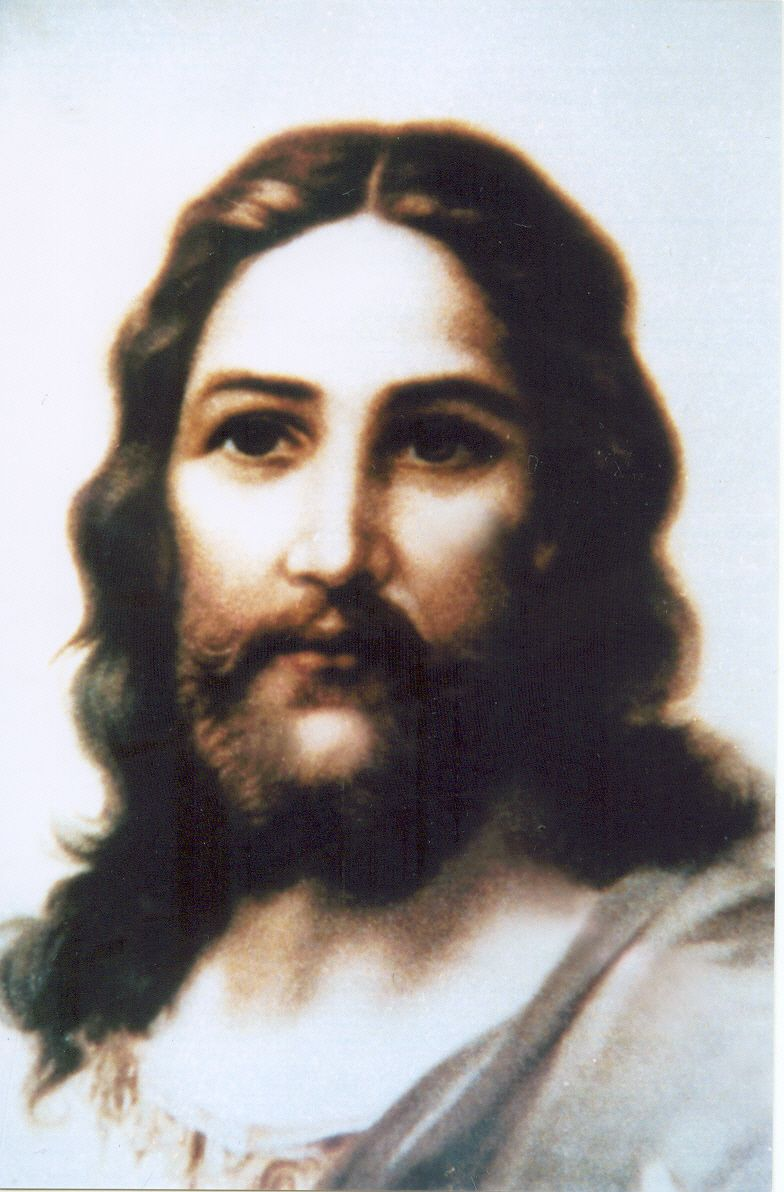
\includegraphics[scale=.5]{Cristo}
			\end{center}

		\subsection{Bondade Infinita $ \Rightarrow $ Justi\c{c}a Infinita}
			\begin{flushright}
			\end{flushright}

			\begin{proof}
				A soberana bondade implica a soberana justi\c{c}a, porquanto, se $ \alpha_\omega $ procedesse injustamente ou com parcialidade \emph{numa s\'o circunst\^ancia que fosse}, ou com rela\c{c}\~ao \emph{a uma s\'o de suas criaturas} \cite{criatura}, j\'a n\~ao seria soberanamente justo e, em consequ\^encia, j\'a n\~ao seria soberanamente \emph{bom}. (\cite{genese}, cap. 2, item 14)
			\end{proof}

			A uma Justi\c{c}a $ \infty $ \'e infantil a ideia: \textquotedblleft estou arrependido; logo, acabou minha culpa.\textquotedblright\, Desconsideraria atenuantes e agravantes.

			E vale para n\'os a \href{http://en.wikipedia.org/wiki/Contraposition}{contrapositiva}.

			[*** \href{http://sites.google.com/site/mathspirituality/}{English}]

		\subsection{A Escolha dos Axiomas}\label{escAxiomas}
			\begin{flushright}
			\end{flushright}

			Se partimos do axioma \textbf{A1}: \textbf{a Justi\c{c}a de Deus \'e Infinita}

			\textbf{Primeira} consequ\^encia: o monoencarnacionismo\cite{demomono} o contradiz e, portanto, \'e uma falsidade.

			\begin{flushright}
			\end{flushright}

			Sem reencarna\c{c}\~ao n\~ao h\'a Justi\c{c}a, pois nascem pessoas em ber\c{c}o de ouro e outras ao mesmo tempo\cite{tempo} pobres, feias ou em piores condi\c{c}\~oes.

			\textquotedblleft A cada um ser\'a dado segundo suas obras.\textquotedblright\, Mateus 16, 27 \cite{obras} $ \Rightarrow $ Sendo anterior ao futuro, a obra est\'a no presente ou no passado. Se uma pessoa nasce doente, as obras dela foram feitas numa vida pregressa.

			Isso implica que Deus n\~ao d\'a presente. Nada de gra\c{c}a. Nem esmola.

			\begin{flushright}
			\end{flushright}

			\textbf{Segunda} consequ\^encia: Lei de Progresso e toda a teoria evidente\cite{evidencias} da Evolu\c{c}\~ao.

			Sem a reencarna\c{c}\~ao, como se explicaria a diferen\c{c}a que existe entre o presente estado social\cite{social} e o dos tempos de barb\'arie? Se as almas s\~ao criadas ao mesmo tempo\cite{tempo} que os corpos\cite{demonismo}, as que nascem hoje s\~ao t\~ao novas, t\~ao primitivas, quanto as que viviam h\'a mil anos; acrescentemos que nenhuma conex\~ao haveria entre elas, nenhuma rela\c{c}\~ao necess\'aria; seriam de todo estranhas umas \`as outras. Por que, ent\~ao, as de hoje haviam de ser melhor dotadas por $ \alpha_\omega $, do que as que as precederam? Por que t\^em aquelas melhor compreens\~ao? Por que possuem instintos mais apurados, costumes mais brandos? Por que t\^em a intui\c{c}\~ao de certas coisas, sem as haverem aprendido? Duvidamos de que algu\'em saia desses dilemas, a menos admita que $ \alpha_\omega $ cria almas de diversas qualidades, de acordo com os tempos e lugares, proposi\c{c}\~ao inconcili\'avel com a ideia de uma justi\c{c}a soberana.

			Admiti, ao contr\'ario, que as almas de agora j\'a viveram em tempos distantes; que possivelmente foram b\'arbaras como os s\'eculos em que estiveram no mundo, mas que progrediram; que $\forall$ nova exist\^encia trazem o que adquiriram nas exist\^encias precedentes; que, por conseguinte, as dos tempos civilizados n\~ao s\~ao almas criadas mais perfeitas [Se\c{c}\~ao \ref{serPerfeito}], por\'em que se aperfei\c{c}oaram por si mesmas com o tempo, e tereis a \'unica explica\c{c}\~ao plaus\'ivel da causa do progresso social\cite{social}. (\cite{genese}, cap. 11, item 33)

			\begin{flushright}
			\end{flushright}

            \textbf{A2}: A exist\^encia do ser pensante (\href{http://pt.wikipedia.org/wiki/Ren\%C3\%A9_Descartes}{Descartes}). Quem tem evid\^encias\cite{evidencias} de que n\~ao existe?

		\subsection{Estruturas}\label{estruturas}

			\begin{flushright}
			\end{flushright}

			Duas Verdades encadeadas.

			O universo pode ter duas causas? Sim, desde que estejam de tal forma coordenadas ou subordinadas, que uma causa n\~ao desbanca, nem derruba, nem nega a outra.

			Retiremos a estrutura que coordena ou subordina, e teremos uma estrutura \'unica com tais e tais propriedades.

			Existem leis da mat\'eria, leis da energia. Retiremos a estrutura que gera as diferen\c{c}as, e teremos uma lei \'unica. Existem leis do fluido e leis do esp\'irito; por tr\'as de ambas, existe uma lei coordenada de cria\c{c}\~ao, subordinada a $ \alpha_\omega $.

			Existe uma \'unica ess\^encia com tais e tais propriedades.

			Todos os seres t\^em tais e tais propriedades.

			Cada \'atomo do fluido tem tais e tais propriedades.

			A energia \'e uma estrutura com tais e tais propriedades.

			A mat\'eria \'e um objeto com tais e tais propriedades.

			O ser biol\'ogico se esgota com tais e tais propriedades.

			\begin{flushright}
			\end{flushright}

			Em A G\^enese\cite{genese}, cap. 2, item 16, KARDEC cometeu uma \emph{miscalculation}. Veja a Se\c{c}\~ao \ref{individuality}. Na verdade, ou $ \alpha_\omega $ \'e \'unico, ou h\'a mais de um $ \alpha_\omega $ com mesmas propriedades.

			Uma coisa \'e dizer $ \exists \left\{ x, y \right\} , x = y $. $ \alpha_\omega $ seria uma abstra\c{c}\~ao, absurdo.

			Outra coisa dizer: tenho uma esfera branca $A$ e uma esfera branca $B$, $A \neq B$. $ \alpha_\omega $ est\'a na realidade emp\'irica.

			Seja a esfera $A = \left\{x \in \mathbb{R} ^ n : |x| = 1 \right\} \cong $ Esfera $B \Leftrightarrow A = B + \mathbf{v} \in \mathbb{R} ^ n$.

			Se n\~ao existir espa\c{c}o, $A = B$. Congru\^encia\footnotemark[1] \emph{versus} igualdade. A ess\^encia geom\'etrica est\'a na invari\^ancia por transla\c{c}ao, rota\c{c}ao e reflex\~ao: Seja $T$ uma matriz de rota\c{c}\~ao e $R(X, r)$ a fun\c{c}\~ao que reflete o conjunto de pontos $X$ com rela\c{c}\~ao \`a reta $r$.

			\footnotetext[1]{Caso especial de rela\c{c}\~oes de equival\^encia: $a \sim a; a \sim b \Rightarrow b \sim a; a \sim b \sim c \Rightarrow a \sim c$}

			\begin{align*}
				&X \cong S(X,v) = X + v \\
				&X \cong T(X, \theta) \\
				&X \cong R(X, r) \\
				\therefore &X \cong (R \circ T \circ S) (X, v, \theta, r)
			\end{align*}

			Na topologia, um pires e uma x\'icara sem cabo sao essencialmente iguais. Sou essencialmente igual a $\alpha_\omega$. Tenho a mesma ess\^encia de $\alpha_\omega$, logo Criador = criatura. Tudo \'e um.

			Existe um \'unico tri\^angulo geom\'etrico, \textquotedblleft m\'odulo\textquotedblright\, todas as rota\c{c}\~oes, transla\c{c}\~oes e reflex\~oes. Seja o ser-tri\^angulo $(a,b,c) | c < a + b$. quem \'e o Deus-tri\^angulo?

		\subsection{Forma e Ess\^encia}\label{essencia}
			\begin{flushright}
			\end{flushright}

			Seja o esp\'irito um conceito indefinido. O ser. A ess\^encia.

			Desejo$(\alpha_\omega) = $\,despertar da autoconsci\^encia.

			Se (\cite{le} q. 23, esp\'irito = p.i.? \cite{le} q. 1: $\alpha_\omega = $ inteligencia superior. \cite{le} q. 76, seres inteligentes?) $\Rightarrow$ intelig\^encia \'e essencial.

			O que \'e igual na criatura $s$ e no Criador? Ex: omnipresen\c{c}a.

			Ess\^encia $\epsilon \Rightarrow$ est\'atico $\Rightarrow \epsilon'(t) = 0$.

			Forma $\equiv \urcorner$ ess\^encia $\Rightarrow$ din\^amico. Elementos da forma: instante de cria\c{c}\~ao, consci\^encia... Express\~ao(ser). Teatro.

			A ess\^encia est\'a al\'em do espa\c{c}o e do tempo. Todo o essencial \'e abstrato? A ilus\~ao pode n\~ao ser a nega\c{c}\~ao da ess\^encia. Evolu\c{c}\~ao \'e ilus\~ao? Quais s\~ao as propriedades da ilus\~ao? Existe uma \'unica ilus\~ao com tais e tais propriedades.

			A ess\^encia tem $n$ propriedades. Essas propriedades se tornam indiv\'iduos, objetos. A ess\^encia \'e um objeto.

			Est\'a praticando, desmaterializando. Pr\'atica \'e ilus\~ao? Eu sou a ess\^encia. Eu sou a pr\'atica?

			\'E o que se conserva? \'E o que tem gradiente nulo? $C$ varia em $t$ at\'e certo ponto, mas no ser perfeito, $\mathbf{\nabla} C = 0$. Colapso dimensional \emph{versus} omnipresen\c{c}a.

			$\mathbf{\nabla} G = 0$

		\subsection{Princ\'ipio espiritual}

			\begin{flushright}
			\end{flushright}

			\emph{Al\'em} do espa\c{c}o e do tempo, tudo s\~ao elementos e conjuntos.

			No princ\'ipio, seja o princ\'ipio espiritual e o princ\'ipio flu\'idico.

			Seja $F$ o conjunto \emph{futuro} das criaturas que existir\~ao.

			Seja $S$ o conjunto das criaturas que existem.

			$S \cap F = \emptyset$.

			Sequ\^encia $C_\alpha$. $\forall \alpha$, um conjunto $C \subset F$.

			$S$ varia em $\alpha \Rightarrow$ funciona como tempo divino.

			$S_\alpha := S \cup \{C_\alpha\}$

			$F_\alpha := F - \{C_\alpha\}$

			Mas $S \cup F \cup \{\alpha_\omega\}$ \'e constante e essencial. Seja um ponto.

			\textquotedblleft No princ\'ipio era o n\~ao-ser, que passou a ser.\textquotedblright

			\subsection{Forma}

			\begin{flushright}
			\end{flushright}

			Seja $I$ a fun\c{c}\~ao individualidade [Se\c{c}\~ao \ref{individuality}]. Funciona como $1$ dimens\~ao espacial divina. Curva imersa em $\mathbb{R}^n$.

			\subsection{Princ\'ipio Flu\'idico}

			\begin{flushright}
			\end{flushright}

			Analogamente, seja o n\~ao ser flu\'idico $F$ e o ser flu\'idico $S$. \textquotedblleft No princ\'ipio era o n\~ao fluido, que passou a ser fluido.\textquotedblright

			$\exists$ um espa\c{c}o-tempo para o fluido/perisp\'irito. Seja o espa\c{c}o vetorial $EV_f$.

			O fluido se densificou e se tornou mat\'eria densa. Essa nossa mat\'eria percebida pelos f\'isicos.

			Seja o espa\c{c}o vetorial $EV_d$. Em Einstein, $v = (x,y,z,t)$ tem $\dim 4$. Com curvatura, $\dim EV_d = 5$. Nas cordas com supercordas com membranas, $\dim EV_d \in \{10, 11\}$.

			\subsection{Instante de cria\c{c}\~ao}

			\begin{flushright}
			\end{flushright}

			Seja a criatura simples e ignorante mergulhada em $EV_f$.

			O ser anima o fluido.

			Fluido inerte: $\exists v \in EV_f$ tal que $\nexists s(v)$.

			\subsection{Corpos}\label{corpos} % Fields hehehe

			\begin{flushright}
			\end{flushright}

			Conjunto de pontos perispir\'iticos que um ser ocupa.

			$\forall$ ser, $\exists\,!$ corpo$_f(s_f) = \{v \in EV_f ; s(v) = s_f \}$

			Seja o n\'umero de dimens\~oes espaciais e o n\'umero de dimens\~oes temporais. Para estabelecer a curvatura, \'e necess\'ario que seja maior ou igual: $\dim EV_f \ge e_1 + t_1$.

			An\'alogo a Newton, corpo$_{fe}(s_f)$ representaria as posi\c{c}\~oes do espa\c{c}o ocupadas pelo ser, e o intervalo de tempo de vida seria dado em termos de corpo$_{ft}(s_f)$.

			\subsection{Encarna\c{c}\~ao}

			\begin{flushright}
			\end{flushright}

			Seja $S_p$ o conjunto de seres com perisp\'irito.

			Seja $s_p \in S_p$ mergulhado em $EV_d$.

			$\forall s_d, \exists\,!$ corpo$_d(s_d) = X$, subconjunto de $EV_d$. $\forall X, \exists\,!$ corpo$_f(X) =$ corpo$_f(s_d)$.

			$\dim EV_d \ge e_2 + t_2$

			corpo$_{de}(s_d)$ | posi\c{c}\~oes do espa\c{c}o denso ocupadas pelo ser

			corpo$_{dt}(s_d)$ | possibilita medir o intervalo de tempo de vida org\^anica

			Mat\'eria inerte: $\exists v \in EV_d$ tal que $\nexists s(v)$.

			$\exists v \in EV_d ; \forall s_p, v \notin$ corpo$_d(s_p)$

			$\exists v \in EV_f ; \forall s, v \notin$ corpo$_f(s)$

			\textquotedblleft Naquele local, naquele instante, $\nexists$ fluido quintessenciado.\textquotedblright

			$\exists v \in EV_{fe} ; v \in$ corpo$_{fe}(s_p),$ para um \'unico $s_p(v)$

			$\exists v \in EV_{de} ; v \in$ corpo$_{de}(s_d),$ para [um \'unico] $s_d(v)$ [Cada c\'elula do corpo tem uma alma? Se isso for verdade, $S(v) = \{s_1, s_2, s_3...\}$]

			O ser ocupa espa\c{c}o-tempo denso $\Leftarrow$ est\'a encarnado $\Rightarrow$ um corpo flu\'idico e um corpo denso.

			O desencarnado (somente corpo flu\'idico) pode estar l\'a e aqui. Ent\~ao,

			Seja $EV_d$ \emph{contido isomorficamente} em $EV_f$, da mesma forma que $\mathbb{R} \times \{0\} \subset \mathbb{R}^2 \subset \mathbb{R}^3 \subset \mathbb{R}^4 \subset \mathbb{R}^5 \subset \mathbb{R}^6 \subset \mathbb{R}^7$.

			Quantidade de elementos igual $(\#EV_d = \#EV_f)$, n\'umero de part\'iculas diminui \`a medida que o espa\c{c}o vetorial densifica.

			$\dim EV_d < \dim EV_f$.

			Dois perisp\'iritos ao mesmo tempo: $\exists C_f = \{v \in EV_{fe}\} ; \exists\,!\,s(C_f)$.

			\subsection{Um modelo matem\'atico para a Terceira Revela\c{c}\~ao}

			\begin{flushright}
			\end{flushright}

			Vamos explicar tudo, ent\~ao.

			Seja eu $\in S$, eu' conjunto dos pontos do meu perisp\'irito, eu'' conjunto dos pontos do meu corpo f\'isico.

			Morrer seria perder o eu'' = (eu', 0, 0, ..., 0), onde o n\'umero de zeros \'e $\dim EV_f - \dim EV_d$.

			O cord\~ao de prata est\'a contido em corpo$_f(s_p)$.

			Fecunda\c{c}\~ao.

			Umbrais. Regi\~oes vibrat\'erias. Mundos flu\'idicos. Todos s\~ao consequ\^encias da geometria e das leis f\'isicas em $EV_f$.

			Psicosfera. Aura.

			$\nexists$ milagre. Se eu tirei leite de pedra ontem, ent\~ao o leite materializou ou o fluido da pedra foi modificado at\'e se tornar leite.

			\textquotedblleft estou no mundo, mas n\~ao perten\c{c}o a ele\textquotedblright\, Corpo$_d$(Jesus) $\subset$ atmosfera(Terra), mas $J \notin EV_d$. $J' \in EV_f$. $J \in S$.

			Mat\'eria densa n\~ao \'e involu\c{c}\~ao: \'e materializa\c{c}\~ao.

			\subsection{Outras teorias}

			\begin{flushright}
			\end{flushright}

			Corpo e alma: considerar somente $EV_d$.

			$7$ corpos: considerar $EV_1 \supset EV_2 \supset EV_3 \supset EV_4 \supset EV_5 \supset EV_6 \supset EV_7$

			$\dim EV_7 = n_7 \ge n_{7e} + n_{7t}$

			$\dim EV_6 = n_6 \ge n_{6e} + n_{6t} > n_7$

			etc.

			Monismo.

			Se voc\^e unir esp\'irito e fluido, qual \'e o absurdo?

	\section{O Caminho at\'e a \href{http://sites.google.com/site/mathspirituality/portugues/RefinandoaPerfei\%C3\%A7\%C3\%A3o.ASF?attredirects=0}{Perfei\c{c}\~ao}}\label{caminho}
			\begin{flushright}
			\end{flushright}

		\subsection{Existe uma Verdade Absoluta.}\label{verdade}
			\begin{flushright}
			\end{flushright}

			\begin{proof}
				Se n\~ao existisse, todas as verdades seriam relativas.

				Exemplo: [Se\c{c}\~ao \ref{escAxiomas}].

				Logo, eu existiria e n\~ao existiria ao mesmo tempo\cite{tempo}. \href{http://en.wikipedia.org/wiki/Proof\_by\_contradiction}{Absurdo}.
			\end{proof}

			Seja $\mathbb{V}$ o conjunto das verdades.

			Suponhamos por absurdo que $ \nexists \nu $.

			\begin{align*}
				\forall \nu \in \mathbb{V}, \exists v_2 \in \mathbb{V} ; \nu \neq v_2 \\
				\nu = \mbox{\textquotedblleft Eu existo\textquotedblright}; v_2 = \urcorner \nu
			\end{align*}

			\begin{center}
				\fbox{$ \exists \nu \in \mathbb{V} ; \forall v_2 \in \mathbb{V}, v_2 = \nu $
				}
			\end{center}

			Conhec\^e-la \'e o caminho. Veja \cite{verdade}.

Seja um infinito enumer\'avel de teoremas $p_1 \Rightarrow p_2 \Rightarrow ...$

			\newtheorem{Q3}{Quest\~ao 3}
			\begin{Q3} A Verdade \'e uma generaliza\c{c}\~ao?
			\end{Q3}

			\begin{flushright}
			\end{flushright}

\cite{lm}, q. 301: \textquotedblleft Os erros s\~ao como as pedras falsas, que s\'o um olhar
experiente pode distinguir. (...) Se adotam o erro, \'e que n\~ao est\~ao
bastante adiantados para compreender a verdade.\textquotedblright

		\subsection{N\~ao existe uma primeira criatura.}\label{firstCreature}
			\begin{flushright}
			\end{flushright}

			Fonte: \cite{genese}, cap. 6, item 14.

			\begin{proof}
				Seja $ t $ o eixo $ \mathbb{R} $eal do Tempo \cite{tempo}.

				$ \alpha_\omega $ sempre existiu, desde $ t = - \infty $\footnotemark[1].

        \footnotetext[1]{Desconhecido $ \Rightarrow \infty $ (\cite{le} q. 2)}

				Suponhamos $ t(c) = t_c \in \mathbb{R} $ (C\'eus), o instante de cria\c{c}\~ao da primeira criatura \cite{criatura}.

				\newtheorem{Q4}{Quest\~ao 4}
				\begin{Q4} Um instante de cria\c{c}\~ao $t(s)$ pode ter v\'arios seres?
				\end{Q4}

				\newtheorem{Q5.1}{Q5.1 (Cardinalidade)}
				\begin{Q5.1} Existe um instante m\'inimo?
				\end{Q5.1}

				Ent\~ao $ \alpha_\omega $ ficou sem criar no intervalo $(-\infty, c)$, caracterizando \textquotedblleft muda letargia inativa e infecunda\textquotedblright, \textquotedblleft morte aparente para o Pai eterno que d\'a vida\textquotedblright, \textquotedblleft mutismo indiferente para o Verbo\textquotedblright, \textquotedblleft esterilidade fria e ego\'ista\textquotedblright. \href{http://en.wikipedia.org/wiki/Proof_by_contradiction}{Absurdo}.
			\end{proof}

			Logo, $ \forall $ criatura\footnotemark[1], $ \exists $ outro instante de cria\c{c}\~ao precedente.

			\footnotetext[1]{Lista de S\'imbolos na Se\c{c}\~ao \ref{simbolos}} %para a secao logica e espiritualidade

			$ \forall $ criatura, $ \exists $ infinitas criaturas antes dela.

			\newtheorem{Q5.2}{Q5.2 (Cardinalidade)}
			\begin{Q5.2} A quantidade de criaturas \'e igual \`a cardinalidade dos conjuntos enumer\'aveis (seja $ \mathbb{Q} $), ou maior [Se\c{c}\~ao \ref{continuidade}]?
			\end{Q5.2}

		\subsection{A \href{http://sites.google.com/site/mathspirituality/portugues/Consci\%C3\%AAnciaCr\%C3\%ADstica.ASF?attredirects=0}{Consci\^encia} Cr\'istica \'e o m\'inimo}\label{ccristica}
			\begin{flushright}
			\end{flushright}

			Sejam
			$C_J$ = Consci\^encia Cr\'istica,
			$C_V = $ Conhecer a Verdade,
			$ C_{\mathrm{Self}} = $ Conhecer a si mesmo = 100 \% de Autoconsci\^encia,
			$ C_{\alpha_\omega} $ = Conhecer $ \alpha_\omega $,
			$C_\infty =$ Consci\^encia infinita,
			$P = $ Perfei\c{c}\~ao.

			\fbox{$P \Rightarrow C_{\alpha_\omega} \Rightarrow C_\infty \Rightarrow C_{\mathrm{Self}} \Rightarrow C_V \Rightarrow C_J $
			}

			\begin{proof}
			Jo\~ao 14, 6. [Se\c{c}\~ao \ref{caminho}] $C_V \Rightarrow C_J $

			Jo\~ao\cite{unidade} 14, 7. $C_{\alpha_\omega} \Rightarrow C_J $

			Jo\~ao\cite{verdade} 8, 32. Ser verdadeiramente livre $ = P \Rightarrow C_V $

			Temos $ P \subseteq V \subseteq J \wedge \alpha_\omega \subseteq J$.

			Self cont\'em a ess\^encia [Se\c{c}\~ao \ref{essencia}] de $\alpha_\omega$, logo, est\'a junto a $\alpha_\omega$. Mas $\alpha_\omega \varsubsetneqq $ Self.

			$ \alpha_\omega $ vai al\'em da Verdade, assim como a perfei\c{c}\~ao vai al\'em da consci\^encia [Se\c{c}\~ao \ref{amor}], ainda que infinita.

			Temos:

			$ V \supseteq P $

			$ \infty \varsupsetneqq P $ (Sim, $ \infty $ aqui \'e um conjunto.)

			$ J \supseteq V \varsupsetneqq \mathrm{Self} \varsupsetneqq \alpha_\omega $

			Quem conhece $ \alpha_\omega $, conhece $ \infty $? (i) Quem conhece $ \infty $, conhece $ \alpha_\omega $? (ii)

			(i) Sim. Ou $ \infty \supseteq \alpha_\omega $, ou $ \infty \varsupsetneqq \alpha_\omega \Leftrightarrow \exists x \in \infty - \alpha_\omega $

			(ii) N\~ao podemos aceitar que seja poss\'ivel conhecer algo al\'em de $ \alpha_\omega $, ou seja, \'e falso que $ \alpha_\omega \varsupsetneqq \infty $. Portanto, \'e verdade que $ \alpha_\omega - \infty = \emptyset $.

			Aceitando as duas $(\infty = \alpha_\omega)$, aceitamos que $C_{\alpha_\omega} \Leftrightarrow C_\infty $.

			Caso $ \alpha_\omega $ v\'a al\'em do conhecimento e al\'em do $ \infty: J \supseteq V \varsupsetneqq \mathrm{Self} \supseteq \infty \varsupsetneqq \alpha_\omega \supseteq P$.
			\end{proof}

			\newtheorem{Q6}{Q6}
			\begin{Q6} O que h\'a para se conhecer entre a Verdade e a mim mesmo? O que h\'a entre a consci\^encia cr\'istica e a consci\^encia da Verdade?
			\end{Q6}

		\subsection{Rela\c{c}\~ao criatura/Criador}\label{criaturaCriador}
			\begin{flushright}
			\end{flushright}

			Seja o ser $ s $ e a Evolu\c{c}\~ao\footnotemark[1] $ E $ uma fun\c{c}\~ao que o associa a um n\'umero, inicialmente em $ \mathbb{\bar{R}} = \mathbb{R} \cup \left\{\pm \infty\right\} $.

			\footnotetext[1]{A grandeza est\'a bem definida?}

			Por abuso de nota\c{c}\~ao, Im $(E: S \rightarrow \mathbb{\bar{R}}) = \mathbb{E} $.

			\newtheorem{Q5.E}{Quest\~ao 5.E (Cardinalidade)}
			\begin{Q5.E} Ou $E(s)$ vai at\'e um topo $ E_M $, ou at\'e $ \infty $.
			\end{Q5.E}

			\newtheorem{Q7.E}{Q7.E (Mensurabilidade)}
			\begin{Q7.E} $E$ \'e mensur\'avel?
			\end{Q7.E}

			Vamos nos restringir ao Espiritismo e oportunamente passamos \`a descoberta de absurdos ou verdades nos outros casos. Se existirem 500 religi\~oes, eu quero os 500 conjuntos de axiomas [Se\c{c}\~ao \ref{escAxiomas}] e suas consequ\^encias.

			\newtheorem{Q8}{Q8}
			\begin{Q8} \'E poss\'ivel a exist\^encia de duas Verdades [Se\c{c}\~ao \ref{verdade}] distintas? [Se\c{c}\~ao \ref{estruturas}]
			\end{Q8}

			Consideremos o primeiro caso\footnotemark[2], e deixemos $E(\alpha_\omega)$ indefinida.

			\footnotetext[2]{\'e necess\'ario que o supremo do intervalo perten\c{c}a a ele, pois, caso contr\'ario, sempre que um topo fosse atingido, existiria outro topo, e, assim, indefinidamente | isso implica que j\'a estou divergindo do senso comum esp\'irita, que reza: \textquotedblleft sempre se aproximando dele, sem jamais alcan\c{c}\'a-lo\textquotedblright. Uns dizem que a criatura est\'a para $ \alpha_\omega $ assim como $y = 0$ est\'a para $y = \frac{1}{x}$. Ass\'intotas.}

			\newtheorem{R1}{Restri\c{c}\~ao 1}
			\begin{R1} $ E(s) < E_M \Rightarrow s \neq \alpha_\omega $.
			\end{R1}

			Logo, $ E(\alpha_\omega) \ge E_M $, mas se $ E(s) = E_M $, ent\~ao pode ocorrer $s = \alpha_\omega $ ou $ s \neq \alpha_\omega $. Veja a \textbf{R2}.

		\subsection{Dimens\~ao de $E$}\label{amor} %consciencia est\'a apontando pra c\'a
			\begin{flushright}
			\end{flushright}

			Fa\c{c}amos uma cis\~ao entre a evolu\c{c}\~ao da consci\^encia $E_c$ e a evolu\c{c}\~ao do amor $E_a$.

			Liberta\c{c}\~ao das ilus\~oes $ \Rightarrow $ Descoberta da Verdade $ \Rightarrow $ Evolu\c{c}\~ao da Consci\^encia.

			Todas as imperfei\c{c}\~oes morais s\~ao obst\'aculos ao Amor: orgulho, ego\'ismo, vaidade, apego \`a mat\'eria.

			\begin{center}
			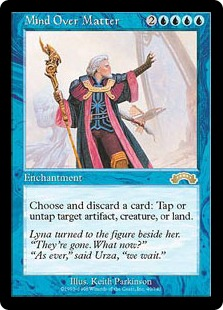
\includegraphics{mind}
			\end{center}

			Todas as virtudes s\~ao filhas do Amor.

			Logo, Liberta\c{c}\~ao Moral $ \Rightarrow $ Aquisi\c{c}\~ao de virtudes $ \Rightarrow $ Evolu\c{c}\~ao do Amor.

			Sejam $ E_c $, $ E_a $ e o Amor $A$ fun\c{c}\~oes de mesmo dom\'inio e contradom\'inio que $E$.

			\newtheorem{Q5.A}{Q5.A (Cardinalidade)}
			\begin{Q5.A} Ou $A(s)$ vai at\'e um topo $ A_M $, ou at\'e $ \infty $.
			\end{Q5.A}

			\newtheorem{Q7.A}{Q7.A}
			\begin{Q7.A} $A$ \'e mensur\'avel?
			\end{Q7.A}

			%isso era para estar na aproximacao classica, juntamente com a eternidade da alma [t_c, \infty)

			\newtheorem{Q9}{Q9 (N\~ao increa\c{c}\~ao)}
			\begin{Q9} Ou o ser possui um ponto de cria\c{c}\~ao, que pode estar no $ -\infty $, ou o ser sempre existiu.
			\end{Q9}

			Em se tratando do Criador, al\'em de $ A_M $, existiria desamor. Estamos supondo que o Amor da criatura evolui de um valor inicial at\'e $ \infty \ $, ent\~ao:

			\begin{align*}
				E_a(s) = E_{a_M} &\Rightarrow A(s) = \infty; \\
				E_a(s) < E_{a_M} &\Rightarrow A(s) = a \in \mathbb{R}.
			\end{align*}

			Im $ E_a(s) = [E_{a_0}, E_{a_M}] $ e o esbo\c{c}o do gr\'afico $ A \times E_a $ \'e semelhante ao \href{http://mathworld.wolfram.com/InverseTangent.html}{arco de tangente}.

			Se $E_a$ for injetiva $\Rightarrow$ rec\'iproca.

			Podemos considerar o amor como um raio $ r_a $, variando em $ [r_{a_0}, \infty] $. (\cite{genese} cap. 14, item 22)

			Seja a Consci\^encia $C$ an\'aloga a $A$. Veja a Se\c{c}\~ao \ref{caracEc}.

			\newtheorem{Q5.C}{Q5.C (Cardinalidade)}
			\begin{Q5.C} Ou $C(s)$ vai at\'e um topo $ C_M $, ou at\'e $ \infty $.
			\end{Q5.C}

			\newtheorem{Q7.C}{Q7.C}
			\begin{Q7.C} $C$ \'e mensur\'avel?
			\end{Q7.C}

			\begin{align*}
				E_c(s) = E_{c_M} &\Rightarrow C(s) = \infty; \\
				E_c(s) < E_{c_M} &\Rightarrow C(s) = c \in \mathbb{R}.
			\end{align*}

			Im $ E_c(s) = [E_{c_0}, E_{c_M}] $ e o raio de consci\^encia $ R_c = [r_{c_0}, \infty] $.

			\newtheorem{Q10}{Q10}
			\begin{Q10} N\'umeros transfinitos: Talvez o $ \infty $ de $A$ n\~ao seja o mesmo $ \infty $ de $C$. Talvez $ \dim(A) > \dim(C) $.
			\end{Q10}

			Ou seja, talvez n\'os criaturas possamos amar, mais do que possamos saber.

		\subsection{O Ser Perfeito}\label{serPerfeito}
			\begin{flushright}
			\end{flushright}

			Sejam a fun\c{c}\~ao vetorial $ \mathbf{E} = \mathbf{E} (s) = E_a(s) \mathbf{i} + E_c(s) \mathbf{j} $ e o topo da evolu\c{c}\~ao

			\begin{align}
				\mathbf{\Pi} &= \left(\Pi_a, \Pi_c\right) = \left(E_{a_M} = E_{c_M}\right)
			\end{align}

			Ilustra\c{c}\~ao para os conjuntos:

			\begin{equation*}
				\left.\begin{aligned}
					\mathbb{S} \rightarrow \mathbb{A} \subset \mathbb{R} \rightarrow \mathbb{E}_a \subset \mathbb{R} \\
					\mathbb{S} \rightarrow \mathbb{C} \subset \mathbb{R} \rightarrow \mathbb{E}_c \subset \mathbb{R}
				\end{aligned}
				\right\}
				\rightarrow \mathbb{E} \subset \mathbb{R}^2
			\end{equation*}

			\newtheorem{D1}{Defini\c{c}\~ao}
			\begin{D1} $s$ \'e perfeito $ \Leftarrow A(s) = \infty \wedge C(s) = \infty $.
			\end{D1}

			\newtheorem{K}{Kierkegaard \cite{kierk}}
			\begin{K}
				Logo, $s$ \'e perfeito $ \Rightarrow \mathbf{E}(s) = \mathbf{\Pi} $. Isso implica que $ s \neq \alpha_\omega $? (Veja a \textbf{R1} e a \textbf{R2}.)
			\end{K}

			Pela indefini\c{c}\~ao de $E(\alpha_\omega)$, Deus pode ser perfeito ou mais-que-perfeito. Em $\mathbf{\Pi}$ se confundem $\alpha_\omega$ e outros seres perfeitos, sem distin\c{c}\~ao.

			(Ser perfeito $ \Leftrightarrow $ Estar no topo da evolu\c{c}\~ao) $ \Rightarrow $ Amor $ \infty $.

			\begin{align*}
			    E(s) < \Pi \Rightarrow E_a(s) < E_{a_M} \vee  E_c(s) < E_{c_M} \Rightarrow s \neq \alpha_\omega
			\end{align*}

			Logo, $ E(s) < \Pi \Rightarrow s \neq \alpha_\omega \Rightarrow E(s) \le \Pi $.

			Mais do que isso, estamos sem uma condi\c{c}\~ao suficiente para que a criatura seja perfeita.

			\newtheorem{Q11}{Q11 (Natureza de $\alpha_\omega$)}
			\begin{Q11} Ou o ser que chegou ao topo da evolu\c{c}\~ao se iguala a $ \alpha_\omega $, ou Este(a) \cite{generoDeus} tem algum atributo al\'em de todos os das criaturas. Suponhamos o segundo caso (\cite{ese} cap. 17, item 2).
			\end{Q11}

			Seja o ser perfeito $p$.
			\begin{align*}
				A(p) = \infty; \
				C(p) = \infty; \
				E_a(p) = E_{a_M}; \
				E_c(p) = E_{c_M}; \
				\mathbf{E}(p) = \mathbf{\Pi}.
			\end{align*}

			Temos $A(\alpha_\omega) = A(p), C(\alpha_\omega) = C(p)$, e gostar\'iamos que

			\begin{center}
				\fbox{$|E(s)| \le |\mathbf{\Pi}| \Leftrightarrow s \neq \alpha_\omega$
				}
			\end{center}

			\newtheorem{R2}{Restri\c{c}\~ao 2}
			\begin{R2} Basta exigir que
			\end{R2}

			\begin{align}
				E_a(\alpha_\omega) > \Pi_a \vee E_c(\alpha_\omega) > \Pi_c
			\end{align}

			\newtheorem{Q12}{Q12}
			\begin{Q12} $ \mathbf{E}(\alpha_\omega)$ tem algum dentre os 4 formatos seguintes: $ (a, c), (a, \infty), (\infty, c) $ ou $ (\infty, \infty) $.
			\end{Q12}

			\newtheorem{Q5.3}{Q5.3 (Cardinalidade)}
			\begin{Q5.3} Quais atributos do ser perfeito s\~ao finitos e quais s\~ao infinitos?
			\end{Q5.3}

		\subsection{Valores Simplificadores}
			\begin{flushright}
			\end{flushright}

			Podemos tratar esses limites superiores como percentuais de evolu\c{c}\~ao, identificando-os com a unidade, desde que zeremos os valores iniciais. Por outro lado, podemos trabalhar com percentual de perfei\c{c}\~ao:

			\begin{align*}
				E_{a_0} = E_{c_0} &= 0 \\
				\Pi_a = \Pi_c = 1 \Rightarrow |\mathbf{\Pi}| &= \sqrt{2} \Rightarrow \Pi_a^2 + \Pi_c^2 = 2 \Rightarrow \exists \theta \in [0, 2\pi) : \mathbf{\Pi} = \sqrt{2} (\cos \theta, \mbox{sen } \theta) \\
				|\mathbf{\Pi}| &= 1 \Rightarrow \mathbf{\Pi} = (\cos \theta, \mbox{sen } \theta)
			\end{align*}

			\newtheorem{Q5.4}{Q5.4 (Cardinalidade)}
			\begin{Q5.4} Compare $ E_{a_M} $ com $ E_{c_M} $. \'E equivalente a:
			\end{Q5.4}

			\begin{align*}
				\mathrm{Ou}\,\theta < \frac{\pi}{4}, \,\mathrm{ou}\, \theta = \frac{\pi}{4}, \,\mathrm{ou}\, \theta > \frac{\pi}{4}.
			\end{align*}

			Voltando a Cantor (Se\c{c}\~ao \ref{continuidade}), a chave dessa quest\~ao \'e a restri\c{c}\~ao a dois intervalos semi-abertos, definidos na Se\c{c}\~ao \ref{serPerfeito}].

			No gr\'afico $ x = E_a \times E_c = y $, onde vemos a trajet\'oria do ser, pode haver segmentos verticais ou horizontais, indicando que globalmente uma componente pode n\~ao ser fun\c{c}\~ao da outra. Equa\c{c}\~ao do movimento...

			Costuma-se dizer que $E_a$ e $E_c$ funcionam como \textquotedblleft duas asas\textquotedblright\, da evolu\c{c}\~ao. Se isso for verdade,

			\newtheorem{Q13}{Q13}
			\begin{Q13} Qual \'e a restri\c{c}\~ao? Qual \'e o m\'aximo que podemos evoluir a) em $E_a$ sem $E_c$? b) em $E_c$ sem $E_a$?
			\end{Q13}

		\subsection{Aproxima\c{c}\~ao Cl\'assica}
			\begin{flushright}
			\end{flushright}

			A evolu\c{c}\~ao \'e direta no caminho de menor comprimento $L$: reta $r$.

			\begin{align*}
				L &= \sqrt{\Pi_x^2 + \Pi_y^2} \\
				y = f(x) = ax; \ f\left(\Pi_x\right) = \Pi_y \Rightarrow y &=\frac{\Pi_y}{\Pi_x} x
			\end{align*}

			Sejam os pontos de \textquotedblleft mudan\c{c}a de reino\textquotedblright: $ \mathbf{R}_M $ mineral, $ \mathbf{R}_V $ vegetal, $ \mathbf{R}_A $ animal, $ \mathbf{R}_H $ hominal, $ \mathbf{R}_\alpha $ angelical.

			\begin{center}
			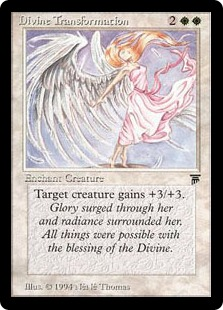
\includegraphics{transformation}
			\end{center}

			\newtheorem{Q14.R}{Q14.R (Conjunto universo)}
			\begin{Q14.R} Determinar uma condi\c{c}\~ao suficiente para que eles existam. Eles est\~ao bem definidos em fun\c{c}\~ao de $s$, ou para todo ser?
			\end{Q14.R}

			\newtheorem{Q5.R}{Q5.R (Cardinalidade)}
			\begin{Q5.R} Determinar $ \#\left\{s \in \mathbb{S} : R(s) = R_0 \right\}$.
			\end{Q5.R}

			\newtheorem{Q15}{Q15 (Involu\c{c}\~ao)}\label{involution}
			\begin{Q15}
				Ou $ \nexists $ involu\c{c}\~ao\footnotemark[1] (\cite{le} q. 118), ou (a partir de certo $ \mathbf{E}_{inv} = (E_a, E_c)_{inv}$ determinado),

				$ \exists $ um raio infinitesimal $ \delta $ at\'e onde o ser pode involuir. Caso 1:
			\end{Q15}

			\footnotetext[1]{Como pode o ser galgar um degrau com tanto esfor\c{c}o, vem a Lei e \~e\~e! derruba. Podem chamar a involu\c{c}\~ao de quarta ou mil\'esima revela\c{c}\~ao que estou com Leon Denis.}

			Para determinado ser $s$, podemos supor $ \mathbf{E}(t) $  a posi\c{c}\~ao dele na senda evolutiva, variando no \emph{tempo} de 0 (cria\c{c}\~ao) at\'e um $ t_\Pi \in \mathbb{T} $ de perfei\c{c}\~ao. (Veja \cite{brennan} Cap. 4, p. 44)

			\newtheorem{Q5.5}{Q5.5 (Cardinalidade)}
			\begin{Q5.5} Ou $ \nexists $ o conceito de tempo, ou $ t_\Pi $ \'e finito, ou $ \infty $\footnotemark[2]. Se for finito, o que $p$ e $ \alpha_\omega $ fazem eternidade afora? O intervalo de tempo \'e aberto ou fechado em $ t_\Pi $? Existe um instante m\'aximo?
			\end{Q5.5}

			\footnotetext[2]{aqui concordo com o \textquotedblleft sem jamais alcan\c{c}\'a-lo\textquotedblright}

			Ent\~ao, $\forall t$, pela n\~ao-involu\c{c}\~ao do amor, $ x'(t) \ge 0 $; pela n\~ao-involu\c{c}\~ao da consci\^encia, $ y'(t) \ge 0 $.

			\newtheorem{Q16}{Q16 (In\'ercia)}
			\begin{Q16} O ser est\'a estacion\'ario $ \Leftarrow \mathbf{E}'(t) = \mathbf{0} $. Isso \'e poss\'ivel?
			\end{Q16}

			Se o movimento \'e inercial:

			\begin{align*}
				\mathbf{E}''(t) &= \mathbf{0} \\
				\mathbf{E}'(t) &= v\mathbf{\hat\Pi} \\
				\mathbf{E}(t) &= vt\mathbf{\hat\Pi} + 0 \\
				\mathbf{E}(t_\Pi) &= vt_\Pi\mathbf{\hat\Pi} = \mathbf{\Pi} \Rightarrow vt_\Pi = |\mathbf{\Pi}| \\
				\mathbf{E}(t) &= \frac{|\mathbf{\Pi}|}{t_\Pi}t\mathbf{\hat\Pi} = \frac{t}{t_\Pi} \mathbf{\Pi}
			\end{align*}

			Se houver 2 seres, pode haver colis\~ao (for\c{c}as, a\c{c}\~ao e rea\c{c}\~ao), massa e gravita\c{c}\~ao, carga e repuls\~ao.

			Intera\c{c}\~ao $(s_1, s_2)$ $\times$ Justi\c{c}a.

			\begin{align*}
				\mathbf{R}_M &= \mathbf{E}\left(t_M\right); \
				\mathbf{R}_V = \mathbf{E}\left(t_V\right); \
				\mathbf{R}_A = \mathbf{E}\left(t_A\right); \\
				\mathbf{R}_H &= \mathbf{E}\left(t_H\right); \
				\mathbf{R}_\alpha = \mathbf{E}\left(t_\alpha\right).
			\end{align*}

			Em $ t_\Pi $, existem saltos nas grandezas, do finito para $ \infty $.

			\begin{center}
				\fbox{
					\begin{minipage}{4cm}{}
						$ A(t) = \infty \Leftrightarrow t \ge t_\Pi $

						$ C(t) = \infty \Leftrightarrow t \ge t_\Pi $
					\end{minipage}
				}
			\end{center}

			\newtheorem{C1}{Conjectura 1}
			\begin{C1} Finito $ \Rightarrow $ Ilus\~ao. Infinitos universos?
			\end{C1}

			\cite{le} 35: Como s\~ao infinitas as criaturas [Se\c{c}\~ao \ref{firstCreature}], todas as somat\'orias sobre $\mathbb{S}$ s\~ao infinitas. Se alguma $\Sigma$ fosse finita, ent\~ao seria limitada. Logo n\~ao existiria \emph{nada} fora dos tais limites. Como o \emph{nada} n\~ao existe, est\'a provado.

		\newtheorem{Q5.t0}{Q5.t0 (Cardinalidade)}
			\begin{Q5.t0} Pir\^amide: determinar a quantidade de seres tais que $ \Delta t = t_\alpha - t_H = t_0 $, dado. Determinar $ \inf \Delta t, \sup \Delta t$.
			\end{Q5.t0}

			Na exist\^encia de duas massas $m_1$ e $m_2$, segundo Newton, existe $G(U_m)_t = 0$. Uma constante de gravita\c{c}\~ao do universo material.

			Portanto, para todo $s_1$ e $s_2$, existe $G(U_s)_t = 0$. Gravita\c{c}\~ao espiritual. $C + E = 0 = A + R = F_{12} + F_{21}$. Causa e efeito. A\c{c}\~ao e Rea\c{c}\~ao.

			$\mathbf{\nabla} G = 0$	[Se\c{c}\~ao \ref{essencia}]

			\begin{flushright}
			\end{flushright}

			Sejam os pontos de \textquotedblleft mudan\c{c}a de escala\textquotedblright: $ \mathbf{E}_I $ esp\'irito impuro, $ \mathbf{E}_L $ esp\'irito leviano, $ \mathbf{E}_F $ esp\'irito pseudo-s\'abio, $ \mathbf{E}_N $ esp\'irito neutro, $ \mathbf{E}_B $ esp\'irito batedor ou perturbador, $ \mathbf{E}_\beta $ esp\'irito ben\'evolo, $ \mathbf{E}_S $ esp\'irito s\'abio, $ \mathbf{E}_W $ esp\'irito de sabedoria, $ \mathbf{E}_\Sigma $ esp\'irito superior, $ \mathbf{E}_U $ esp\'irito puro (\cite{le} q. 100 a 113).

			\newtheorem{Q14.E}{Q14.E}
			\begin{Q14.E} Determinar uma condi\c{c}\~ao suficiente para que eles existam.
			\end{Q14.E}

			\begin{align*}
				\mathbf{E}_I &= \mathbf{E}\left(t_I\right); \
				\mathbf{E}_L = \mathbf{E}\left(t_L\right); \\
				\mathbf{E}_F &= \mathbf{E}\left(t_F\right); \
				\mathbf{E}_N = \mathbf{E}\left(t_N\right); \\
				\mathbf{E}_B &= \mathbf{E}\left(t_B\right); \
				\mathbf{E}_\beta = \mathbf{E}\left(t_\beta\right); \\
				\mathbf{E}_S &= \mathbf{E}\left(t_S\right); \
				\mathbf{E}_W = \mathbf{E}\left(t_W\right); \\
				\mathbf{E}_\Sigma &= \mathbf{E}\left(t_\Sigma\right); \
				\mathbf{E}_U = \mathbf{E}\left(t_U\right).
			\end{align*}

		\subsection {Evolu\c{c}\~ao dos Mundos}
			\begin{flushright}
			\end{flushright}

			Sejam os pontos de \textquotedblleft mudan\c{c}a de mundo\textquotedblright: $ \mathbf{M}_P $ mundo primitivo, $ \mathbf{M}_E $ mundo de expia\c{c}\~oes e provas, $ \mathbf{M}_R $ mundo de regenera\c{c}\~ao, $ \mathbf{M}_D $ mundo ditoso, $ \mathbf{M}_C $ mundo celeste ou divino (\cite{ese} cap. 3, item 4).

			\emph{G\^enesis 3, 24. \textquotedblleft O anjo que, empunhando uma espada flamejante, veda a entrada do para\'iso simboliza a impossibilidade\cite{possibilidades} em que se acham os Esp\'iritos dos mundos inferiores, de penetrar nos mundos superiores, antes que o mere\c{c}am pela sua depura\c{c}\~ao.\textquotedblright\,\cite{genese}, cap. 12, item 23.}

			\begin{center}
			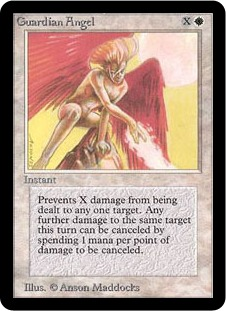
\includegraphics{angel} 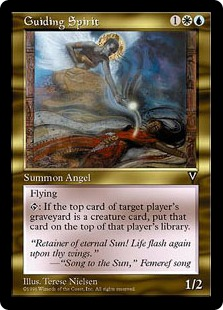
\includegraphics{guiding}
			\end{center}

			\emph{Muita gente por a\'i est\'a com esta carta vermelha se resolvendo. Os detentos\cite{crime} v\~ao para outra pris\~ao e a Terra\cite{Terra} \'e promovida a escola.}

			\begin{center}
			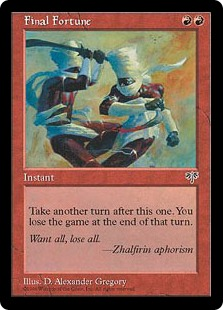
\includegraphics{ff}
			\end{center}

			\emph{A Terra\cite{Terra} est\'a deixando de ser um mundo de provas e expia\c{c}\~oes para ser um mundo de regenera\c{c}\~ao (\cite{ese}, cap. 3, itens 3 a 5).}

Logo, o bem precisa sobrepujar o mal dentro de cada ser. Caso contr\'ario, transfer\^encia. \textquotedblleft o bem
prevalecer\'a sobre o mal\textquotedblright. KARDEC, Allan. \textbf{O Que \'E o Espiritismo}. 53ª ed. Rio de Janeiro,
RJ: FEB, 2005. Cap\'itulo II (No\c{c}\~oes elementares de Espiritismo), item 100 (Consequ\^encias do Espiritismo).

			\begin{center}
			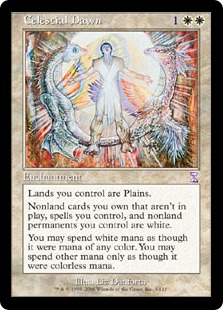
\includegraphics{dawn}
			\end{center}

			\newtheorem{Q14.M}{Q14.M}
			\begin{Q14.M} Determinar uma condi\c{c}\~ao suficiente para que eles existam.
			\end{Q14.M}

			\begin{align*}
				\mathbf{M}_P &= \mathbf{E}\left(t_P\right); \
				\mathbf{M}_E = \mathbf{E}\left(t_E\right); \
				\mathbf{M}_R = \mathbf{E}\left(t_R\right); \\
				\mathbf{M}_D &= \mathbf{E}\left(t_D\right); \
				\mathbf{M}_C = \mathbf{E}\left(t_C\right).
			\end{align*}

			\newtheorem{Q5.M}{Q5.M (Cardinalidade)}
			\begin{Q5.M} Determinar $ \#\left\{s \in \mathbb{S} : M(s) = M_0 \right\}$.
			\end{Q5.M}

			\newtheorem{Q5.MR}{Q5.MR (Cardinalidade)}
			\begin{Q5.MR} Determinar $ \#\{s \in \mathbb{S} : M(s) = M_0 \wedge R(s) = R_0 \}$.
			\end{Q5.MR}

		\subsection{Aproxima\c{c}\~ao Relativ\'istica}\label{relativistica}
			\begin{flushright}
			\end{flushright}

			Se existir uma velocidade m\'axima c, ent\~ao
			\begin{align*}
				\inf(t_\Pi) = \tau = \frac{L}{c}.
			\end{align*}

			Sabemos por \href{http://pt.wikipedia.org/wiki/Albert_Einstein}{Einstein} que a mat\'eria cria um campo gravitacional \`a sua volta que define a curvatura, a geometria do espa\c{c}o-tempo da vizinhan\c{c}a.

			Defina-se assim a geometria perispir\'itica.

			Vamos buscar o espa\c{c}o e o tempo para o perisp\'irito. Qual \'e a curvatura? Quais leis s\~ao iguais \`as nossas? Quais s\~ao diferentes?

			Definir Volume(perisp\'irito). Densidade$(s) < \rho_0 \Rightarrow s$ \'e regenerado.

			Num racioc\'inio simplista, seja a curvatura $k$ proporcional \`a densidade de mat\'eria $= \frac{m}{V}$. Logo, $k$(perisp\'irito) $< k$(mat\'eria).

			Na relatividade restrita, o verdadeiro tempo \'e $\frac{1}{t - t_0}$, que no referencial do fotonzinho \'e zero. A verdadeira dist\^ancia \'e $x - x_0$, que em $v = c$ \'e zero. A verdadeira massa [Se\c{c}\~ao \ref{materializacao}] \'e $\frac{1}{m - m_0}$, que para a luz \'e zero. Qual a curvatura para a massa zero? Matem\'aticos adoram curvatura zero. Qual a dimens\~ao do hiperplano?

			Seja $f$(perisp\'irito) $\propto \frac{1}{f'} = \frac{1}{m} \frac{h}{c^2}$. Seja a frequ\^encia cerebral $f: J = \left[t_N, t_T \right] \rightarrow \mathbb{F}$ variando do nascimento ao t\'umulo. E seja a extens\~ao cont\'inua $F: \left[t_C, \infty \right] \rightarrow \mathbb{F}$ da cria\c{c}\~ao at\'e a eternidade, tal que $f = F\,|_J$.

			$\min f$(reino) define em que tipo de reino est\'a o ser [Teorema \ref{involution}]. O ser pode em sua \'ultima encarna\c{c}\~ao como ser humano (p. ex.) evoluir mais que o m\'inimo para reencarnar no reino angelical:

			\begin{align*}
				0 < f(R_M) \le &f(s) < f(R_V) \Rightarrow s \in R_M \\
				f(R_V) \le &f(s) < f(R_A) + \delta \Rightarrow s \in R_V \\
				f(R_A) \le &f(s) < f(R_H) + \delta \Rightarrow s \in R_A \\
				f(R_H) \le &f(s) < f(R_\alpha) + \delta \Rightarrow s \in R_H \\
				f(R_\alpha) \le &f(s) < f_U + \delta \Rightarrow s \in R_\alpha \\
				f_U \le &f(s) \Rightarrow s \mathrm{\,sem\,necessidade\,de\,reeencarnar}
			\end{align*}

			O objetivo do ser humano \'e alcan\c{c}ar $f(R_\alpha)$. Veste nupcial\cite{batista}.

			$\min f$(atmosfera mundo) define em que tipo de mundo est\'a o ser, a menos de miss\~oes. O ser pode em sua \'ultima encarna\c{c}\~ao na Terra (p. ex.) evoluir mais que o m\'inimo para reencarnar em um mundo melhor:

			\begin{align*}
				0 < f(M_P) \le &f(s) < f(M_E) \Rightarrow s \in M_P \\
				f(M_E) \le &f(s) < f(M_R) + \delta \Rightarrow s \in M_E \\
				f(M_R) \le &f(s) < f(M_D) + \delta \Rightarrow s \in M_R \\
				f(M_D) \le &f(s) < f(M_C) + \delta \Rightarrow s \in M_D \\
				f(M_C) \le &f(s) < f_U + \delta \Rightarrow s \in M_C \\
				f_U \le &f(s) \Rightarrow s \mathrm{\,sem\,necessidade\,de\,reeencarnar}
			\end{align*}

			A meta do terrestre na transi\c{c}\~ao \'e alcan\c{c}ar $f(M_R)$. Veste nupcial\cite{batista}.

			Origem$(U)$: Suponhamos $\underset{(x,y,z,w) \rightarrow \mathbf{0}}{\operatorname{\lim}} f(x^2 + y^2 + z^2 + w^2) = L.$

			Conjectura: em um buraco-negro, $\Delta w > 0$. Em algum outro lugar do universo, uma montanha na quarta dimens\~ao: $\Delta w < 0$.

			A Terra era plana e se fechou sobre si mesma. O Universo era um hiperplano 3D e se fechou sobre si mesmo. Todas as bolhas devem se fechar sobre si mesmas. Todas as membranas devem se fechar sobre si mesmas. Todos os infinitos universos devem se fechar sobre si mesmos. Toda a infinita cria\c{c}\~ao deve ter como centro um Deus infinitamente bom e justo.

			\emph{Dizem que a f\'isica qu\^antica est\'a em um momento estranho, dentro de um buraco negro, talvez. \textbf{Exemplo infantil}: seria poss\'ivel a exist\^encia de um outro universo, que tenha um ponto inicial \textbf{como o nosso}, mas que o tempo\cite{tempo} \textbf{flua} em sentido contr\'ario. O que \'e futuro para n\'os, seria passado \textbf{ali}.}

A consequ\^encia prim\'aria, a consequ\^encia imediata de se
adotar as duas t\~ao citadas teorias acima \'e a igualdade, \'e encarar a
natureza como um bicho de tr\^es faces | part\'icula, energia e onda.

O f\'isico \'e o cara que despreza. Come\c{c}a pelo atrito. Considere uma vaca
quadrada. A f\'isica qu\^antica despreza uma barreira infinita e o el\'etron
penetra.

Existe uma probabilidade d$\Psi$ de
Santa Claus estar descendo agora por uma lareira com uma coca-cola na
m\~ao.
Einstein desprezou a qu\^antica inteira, porque existe uma probabilidade d$\Psi$ de $v > c$.

Existe uma probabilidade d$\Psi$ de a
 m\'aquina de Carnot ser sobrepujada.

Logo, eu prefiro acreditar que a ess\^encia da qu\^antica \'e desprezar $\Psi < \epsilon$, para $\epsilon$ adequadamente pequeno.

Agora suponhamos que os n\'umeros racionais s\~ao perfeitos e que
quanticamente n\~ao existem n\'umeros reais. Logo, tudo \'e perfeito.

		\subsection{Qual \'e a Lei?}\label{leiPerfeicao}
			\begin{flushright}
			\end{flushright}

			Uma quantidade finita de equa\c{c}\~oes diferenciais sobre os pontos-esp\'iritos, talvez.

			Caso sejamos o ser na origem e nossa Motiva\c{c}\~ao Natural seja atingir $ \mathbf{\Pi} $...

			\newtheorem{Q17}{Q17 (Atra\c{c}\~ao)}
			\begin{Q17} Somos atra\'idos por uma for\c{c}a no sentido de $ \mathbf{\Pi} $? Gravitacional, pois n\~ao repele.
			\end{Q17}

			\'E necess\'ario esfor\c{c}o para sair da reta $r$.

			Definir essa for\c{c}a \textbf{F}.

			\newtheorem{Q18}{Q18 (For\c{c}a)}
			\begin{Q18} Se partimos de $ A \in r $ at\'e atingir $ B \notin r $, o que acontece durante a realiza\c{c}\~ao do esfor\c{c}o?
			\end{Q18}

			Em \cite{capela}, h\'a $t_1 < t_2 < t_3$. Em $t_1, E_c > E_a$. Ex\'ilio: $M(t_2) < M(t_1)$. Quando $E_a > \underset{s \in M(t_1)}{\operatorname{\min}} E_a$, ocorre a volta do ex\'ilio: $M(t_3) = M(t_1)$. [Se\c{c}\~ao \ref{materializacao}]

			\newtheorem{Q19}{Q19}
			\begin{Q19} Se o nosso esfor\c{c}o cessa, o que vem a seguir: muda nossa dire\c{c}\~ao para $ \mathbf{\Pi} - \mathbf{B} $, ou voltamos a $ C \in r $?
			\end{Q19}

			%new
			Acelera\c{c}\~ao constante? \textbf{F} decresce linearmente com o tempo?

			\begin{align*}
			\mathbf{F} = \mathbf{F} - \left(F_{x_M}, F_{y_M}\right) \frac{1}{t_f} t
			\end{align*}

			Sempre que \textbf{F} \'e fun\c{c}\~ao s\'o de t,

			\begin{align*}
				\mathbf{a} &\equiv \mathbf{F} / m \\
				\mathbf{F}(t) &= m \mathbf{r}''(t) \\
				\mathbf{r}'(t) &= \frac{1}{m} \int \mathbf{F} \mathrm{d}t + \mathbf{v_0} \\
				\mathbf{r}(t) &= \frac{1}{m} \iint \mathbf{F} \mathrm{d}t \mathrm{d}t + \mathbf{v_0} t + \mathbf{r_0}
			\end{align*}

			Talvez exista \textbf{F(r)}. Contorno: $ x(t_0) = C_x; x(t_f) = B_x $

			\begin{align*}
				\Delta x &= x_f - x_0 \\
				F(x) &= - \frac{F_0}{\Delta x} (x - x_f) = m x'' \\
				x'' &= -Dx + E; \ D = \frac{F_0}{m \Delta x}; \ E = \frac{F_0}{m \Delta x} x_f \\
				E = 0 \Rightarrow x &= c_1 \mbox{sen }(t \sqrt{D}) + c_2 \cos (t \sqrt{D}) \\
				x' &= \sqrt{D} c_1 \mbox{sen }(t \sqrt{D}) - \sqrt{D} c_2 \cos (t \sqrt{D}) \\
				x'' &= -D c_1 \mbox{sen }(t \sqrt{D}) - D c_2 \cos(t \sqrt{D}) = -Dx
			\end{align*}

			N\~ao homog\^enea $\Rightarrow$...

			Ser\'a que $y,z, \mathbf{r}$ vir\~ao naturalmente?

			\newtheorem{Q20}{Q20}
			\begin{Q20} Qual \'e a dist\^ancia entre $ \mathbf{\Pi} $ e $ \mathbf{E}(\alpha_\omega )$? Se \'e transpon\'ivel, o absurdo seria a exist\^encia de mais [Se\c{c}\~ao \ref{epistemologia}] de um deus? \ref{unicidade}
			\end{Q20}

		\subsection{Individualidade}\label{individuality}
			\begin{flushright}
			\end{flushright}

			Sejam os seres perfeitos $ p_1 $ e $ p_2 $ e a fun\c{c}ao individualidade: $ I: \mathbb{S} \rightarrow \mathbb{I} \in \mathbb{R}$. Todos s\~ao criados iguais $ \Rightarrow $ Todos se tornar\~ao iguais.

			A individualidade cont\'inua pode variar em $(\alpha, \beta) \subset \mathbb{R}$ sem igualar-se a ningu\'em. Definimos

			\begin{align*}
				I(s_1) &= I(s_2) \Leftrightarrow s_1 \cong s_2 \\
				I'(t) &= 0
			\end{align*}

			Ou vale a const\^ancia acima, ou temos $I(s, t)$. Ou seja, dados 2 seres diferentes $s_1$ e $s_2$,

			\newtheorem{Q21.s}{Q21.s}
			\begin{Q21.s} $I(s_1)$ e $I(s_2)$ podem ser sempre iguais, sempre diferentes, iguais somente na cria\c{c}\~ao e na perfei\c{c}\~ao, ou ora iguais e ora diferentes. Caso 2:
			\end{Q21.s}

			Em ess\^encia [Se\c{c}\~ao \ref{essencia}], \'e a carteira de identidade espiritual: $\forall s_1, t_1, s_2, t_2, I(s_1, t_1) \neq I(s_2, t_2)$.

			\begin{align*}
				&s \ncong s_2, \forall s_2 \Rightarrow \alpha_\omega \ncong s_2 \\
				\exists ! &s \Rightarrow \exists ! \alpha_\omega
			\end{align*}

			Seja $ \mathbb{S} \cong \mathbb{I} $, i.e., sempre que falarmos de um ser, estamos nos referindo \`a sua individualidade.

			\newtheorem{Q21.p}{Q21.p (Desigualdade de individualidades)}
			\begin{Q21.p} Ou $ I(p_1) = I(p_2) $, ou $ I(p_1) \neq I(p_2) $. [Se\c{c}\~ao \ref{leiIgualdade}]
			\end{Q21.p}

			Tratamento igual por n\'ivel evolutivo.

			\newtheorem{Q22.p}{Q22.p (Tri\^angulo)}
			\begin{Q22.p} S\~ao iguais as rela\c{c}\~oes entre cada $ p_i $ e $ \alpha_\omega $?
			\end{Q22.p}

			Sejam os seres rec\'em-criados $ j_1 $ e $ j_2 $. Seu tempo de vida \'e d$t$. M\^onada.

			\newtheorem{Q21.j}{Q21.j}
			\begin{Q21.j} Ou $ I(j_1) = I(j_2) $, ou $ I(j_1) \neq I(j_2) $.
			\end{Q21.j}

			\newtheorem{Q22.j}{Q22.j}
			\begin{Q22.j} S\~ao iguais as rela\c{c}\~oes entre cada $ j_i $ e $ \alpha_\omega $?
			\end{Q22.j}

			Talvez n\~ao seja poss\'ivel considerar um ser separadamente, como \textquotedblleft part\'icula\textquotedblright.

			\newtheorem{Q5.6}{Q5.6 (Cardinalidade)}
			\begin{Q5.6} $I(s) \in \mathbb{Q}^n$? $I(s) \in \mathbb{R}^n$? Determinar $n$.
			\end{Q5.6}

			\newtheorem{Q5.A0}{Q5.A0 (Cardinalidade)}
			\begin{Q5.A0} Determinar $ \#\left\{s \in \mathbb{S} : A(s) = A_0 \right\}$.
			\end{Q5.A0}

			\newtheorem{Q5.C0}{Q5.C0 (Cardinalidade)}
			\begin{Q5.C0} Determinar $ \#\left\{s \in \mathbb{S} : C(s) = C_0 \right\}$.
			\end{Q5.C0}

			\newtheorem{Q23}{Q23 (Mudan\c{c}a de universo ao mesmo tempo)}
			\begin{Q23} Ou $ t_x = t'_x $, ou $ t_x < t'_x $, ou $ t_x > t'_x, \forall x \in \left\{ \Pi, \, M, \, V, \, A, \, H, \, \alpha, \, P, \, E, \, R, \, D, \, C, \, I, \, L, \, F, \, N, \, B, \, \beta, \, S, \, W, \, \Sigma, \, U\right\}$.
			\end{Q23}

			Quando $t_x(s_1) > t_x(s_2) \wedge M(s_1) > M(s_2)$, ocorre de $s_1$ voltar como mission\'ario para ajudar $s_2$.

			...onda/part\'icula, energia, entropia, calor, luz, linhas de for\c{c}a, quantiza\c{c}\~ao, $ \Psi(\mathbf{r}, t) $, probabilidades, integral...

			\newtheorem{Q24}{Q24 (Ess\^encia)}
			\begin{Q24} A imutabilidade de $ \alpha_\omega $ se transfere ao ser perfeito. Demonstr\'avel ou refut\'avel? Cada ser perfeito tem quais propriedades? E quais dessas propriedades cada criatura tem desde que jaz criada? O que \'e est\'atico e o que \'e din\^amico no caminho?
			\end{Q24}

			Microcria\c{c}\~oes at\'e cria\c{c}\~ao de gal\'axias.

		\subsection{Penas e Gozos}
			\begin{flushright}
			\end{flushright}

			\begin{center}
			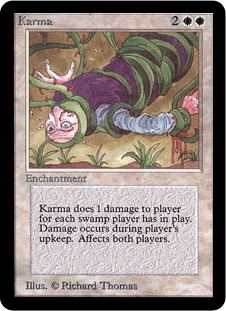
\includegraphics{carma} 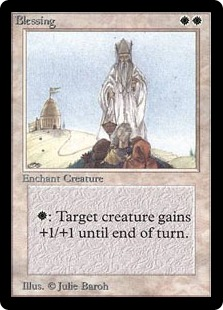
\includegraphics{blessing}
			\end{center}

			A penalidade $ - K(s) $ aumenta atrav\'es do livre-arb\'itrio, diminui atrav\'es de provas e expia\c{c}\~oes.

			\newtheorem{Q8.K}{Q8.K}
			\begin{Q8.K} $K$ \'e mensur\'avel?
			\end{Q8.K}

			Toda penalidade \'e finita. Para um ser em particular, precisamos provar que

			\newtheorem{C2t}{C2$(t)$}
			\begin{C2t} $ \lim K(t) $ n\~ao \'e $ - \infty $ nem em $ t = t_0 $, nem quando $ t \rightarrow \infty $. ($\Leftarrow$ Continuidade)
			\end{C2t}

			\newtheorem{C2st}{C2$(s,t)$}
			\begin{C2st} $K(s,t)$ possui um m\'inimo absoluto.
			\end{C2st}

			Isso ser\'a imediato $ \Leftarrow \forall $ ser, valer $C2(t)$.

			Tamb\'em \'e consequ\^encia de
			\begin{align*}
				\mathbf{\nabla} K(s,t) = \mathbf{0} = \left(\frac{\mathrm{d}K}{\mathrm{d}I}, \frac{\mathrm{d}K}{\mathrm{d}t}\right).
			\end{align*}

			\newtheorem{Q5.K0}{Q5.K0 (Cardinalidade)}
			\begin{Q5.K0} Determinar $ \#\left\{s \in \mathbb{S} : K(s) = K_0 \right\}$.
			\end{Q5.K0}

			\newtheorem{Q25}{Q25}
			\begin{Q25} Ou existe o carma \textquotedblleft positivo\textquotedblright\, indiano, ou $ K(s, t) \le 0 $ (\cite{le} q. 960++). Caso 1:
			\end{Q25}

			Virtudes e v\'icios: $K$(mission\'ario na Terra\cite{Terra}) $ > 0$.

			\newtheorem{Q26}{Q26}
			\begin{Q26} Ou $ \lim K(t) = 0 $, ou $ 0 < \lim K(t) = k_\Pi \in \mathbb{R} $, ou $ \lim K(t) = \infty $.
			\end{Q26}

			Aqui estamos imaginando se o ser tem cr\'edito e d\'ebito, ou seja, as aquisi\c{c}\~oes, a felicidade do ser.

			$ \lim K(t) = 0 \Rightarrow \nexists $ regenera\c{c}\~ao(ser). Absurdo.

			Lei imut\'avel $ \nRightarrow $ Pena definida e irrevers\'ivel.

			Dura\c{c}\~ao das penas $ \propto $ Comportamento$(s)$ (\cite{ese}, cap. 27, itens 20-21)

			Aplica\c{c}\~ao da pena: ou diretamente por $\alpha_\omega$, ou uma hierarquia.

			Diretamente $\nRightarrow$ injusti\c{c}a, mas viola a imutabilidade de $\alpha_\omega$.

			$K(s) = $ resultante(bem, mal, $s$). Hist\'orico: na mem\'oria(ser) (consciente ou inconsciente\cite{Freud}) est\~ao suas a\c{c}\~oes, as imposi\c{c}\~oes da Lei e o que ainda falta de rea\c{c}\~oes.

			Defina: tudo o que fa\c{c}o tem um $K$(a\c{c}\~ao) $\Rightarrow$ Recebo $K$, $2K$ ou $3K$?

			Defina: amor $\times$ dor.

			Todo mundo conhece algu\'em que faz coisas boas $K_+$ e coisas ruins $K_-$. A fim de impedir a inconsist\^encia $\lim K_+ - K_- = \infty$, definimos:

			\begin{align*}
				\dim K &= 2 \Rightarrow K = (K_+, K_-) \\
				K_+ &\ge 0 \\
				K_- = P &\le 0 \\
				\lim K_+ &= \infty \\
				\lim K_- &= 0
			\end{align*}

			Sofrimento $\Rightarrow \Delta K_- > 0 \Rightarrow $ Evolu\c{c}\~ao. Evolu\c{c}\~ao $\Rightarrow \Delta A > 0 \vee \Delta C > 0 \vee \Delta K_- > 0$.

			$K$(reinos):

			\begin{align*}
				&K(R_M) = (0,0); \\
				&K(R_V) = (0,0); \\
				&K(R_A) = (0,0); \\
				&K(R_H) = (a,b); a \in \mathbb{R}_+, b \in \mathbb{R}_- \\
				0 < &K_{+_\alpha} \le K_+(R_\alpha) < K_U; \\
				K_{+_\alpha} < &K_-(R_\alpha) \le 0 \\
				0 < &K_{+_U} < K_+(s) \wedge K_{-_U} < K_-(s) \le 0 \Rightarrow s \mathrm{\,sem\,necessidade\,de\,reeencarnar.}
			\end{align*}

			O objetivo do ser humano \'e alcan\c{c}ar $K_\alpha$. Veste nupcial\cite{batista}.

			Analogamente \`a frequ\^encia [Se\c{c}\~ao \ref{relativistica}], $\min K$(mundo) define em que tipo de mundo est\'a o ser, a menos de miss\~oes. O ser pode em sua \'ultima encarna\c{c}\~ao na Terra (p. ex.) fazer o bem mais que o m\'inimo para reencarnar em um mundo melhor:

			\begin{align*}
				0 > K(M_P) \le &K(s) < K(M_E) \Rightarrow s \in M_P \\
				0 > K(M_E) \le &K(s) < K(M_R) + \delta \Rightarrow s \in M_E \\
				0 < K(M_R) \le &K(s) < K(M_D) + \delta \Rightarrow s \in M_R \\
				K(M_D) \le &K(s) < K(M_C) + \delta \Rightarrow s \in M_D \\
				K(M_C) \le &K(s) < K_U + \delta \Rightarrow s \in M_C \\
				K_U \le &K(s) \Rightarrow s \mathrm{\,sem\,necessidade\,de\,reeencarnar}
			\end{align*}

			A meta do terrestre na transi\c{c}\~ao \'e alcan\c{c}ar $K(M_R)$. Veste nupcial\cite{batista}.

		\subsection{Responsabilidade $\Rightarrow$ Liberdade}\label{respLib}
			\begin{flushright}
			\end{flushright}

			\begin{proof}
				Se n\~ao existisse nenhuma liberdade, a fatalidade abrangeria tudo.

				Se tudo fosse fatal, n\~ao haveria como responsabilizar ningu\'em.	(\cite{ceuinf}, cap. 1, item 10)
			\end{proof}

| Deus teve escolha ao criar o Universo? | Einstein

Maior evolu\c{c}\~ao $\Rightarrow$ maior liberdade, maior quantidade de obriga\c{c}\~oes.

Temos 3 possibilidades: um universo respons\'avel, um universo libertino e um universo fatalista.

1) Deus cumpre (\emph{forever and ever}) sua obriga\c{c}\~ao com requintes de liberdade. (E pela obra se reconhece o artista.)

2) Muita liberdade, pouca responsabilidade. Seria como o pai que faz o filho e n\~ao assume. Imperfeito.

3) A n\~ao-liberdade de Deus. Tudo obrigat\'orio. Nada transcende as Leis Universais. Impossibilidade de ser de outra forma.
Frio. Fico com a (1).

		\subsubsection{Livre-arb\'itrio}
			\begin{flushright}
			\end{flushright}

			Livre-arb\'itrio $\Rightarrow$ interven\c{c}\~ao(ser). Interven\c{c}\~ao direta?

			$E \propto$ raio(escolhas).

		\subsection{\underline{Necessidade da Mat\'eria} | Caracteriza\c{c}\~ao de $ E_a $}\label{materializacao}
			\begin{flushright}
			\end{flushright}

			O ser, ao evoluir moralmente, se desprende da mat\'eria.

			A materializa\c{c}\~ao do ser \'e m\'axima na cria\c{c}\~ao e se anula na perfei\c{c}\~ao, possivelmente antes desta, seja em $ E_{a_U} < \Pi_x $, de Unidade\cite{unidade} $\equiv$ sem mat\'eria.

			\newtheorem{Q2.M}{Q2.M}
			\begin{Q2.M} $M$ \'e mensur\'avel?
			\end{Q2.M}

			\begin{align*}
				M(0) &= M_M; \
				M\left(E_{a_U}\right) = 0 \\
				\int_0^{E_{a_M}} M \,\mathrm{d}E_a &= \int_0^{M_M} E_a \,\mathrm{d}M < E_{a_U} M_M
			\end{align*}

			$\min M$(mundo) define em que tipo de mundo est\'a o ser, a menos de miss\~oes:

			\begin{align*}
				M(M_E) < &M(s) \le M(M_P) \Rightarrow s \in M_P \\
				M(M_R) < &M(s) \le M(M_E) \Rightarrow s \in M_E \\
				M(M_D) < &M(s) \le M(M_R) \Rightarrow s \in M_R \\
				M(M_C) < &M(s) \le M(M_D) \Rightarrow s \in M_D \\
				0 < &M(s) \le M(M_C) \Rightarrow s \in M_C \\
				&M(s) = 0 \Rightarrow s \mathrm{\,sem\,necessidade\,de\,reeencarnar}
			\end{align*}

			Se a Terra est\'a regenerando, cada ser tem que atingir $M(M_R)$. Veste nupcial\cite{batista}.

			No ponto em que n\~ao existir mat\'eria, possivelmente n\~ao haver\'a espa\c{c}o, tampouco tempo. Sejam $E_{se}, E_{st}, E_{set}$ os pontos sem espa\c{c}o, sem tempo e sem espa\c{c}o-tempo.

		\subsection{\underline{O Cord\~ao de Prata}}
			\begin{flushright}
			\end{flushright}

			Seja a liga\c{c}\~ao do perisp\'irito com o corpo f\'isico $L: \mathbb(S) \rightarrow [0, 1] \subset \mathbb{R}$, tal que:

			$s$ est\'a desencarnado $\Rightarrow L(s) = 0$

			$s$ est\'a encarnado $\Rightarrow L(s) = 1$

			No caso do suicida, $0 < L(s) < 1$.

			Consideremos $L(t)$, para um ser \'unico $s$. No nascimento, $\Delta L = 1$. Na morte, $\Delta L \ge -1$.

			Part\'iculas de $EV_f$ que ligam corpo$_d$ a corpo$_f$. [Se\c{c}\~ao \ref{corpos}]

		\subsection{\underline{Ilus\~oes do Ser} | Caracteriza\c{c}\~ao de $ E_c $}\label{caracEc}
			\begin{flushright}
			\end{flushright}

			O ser percebe Verdades $V$ e ilus\~oes $F$.

			Seja a Percep\c{c}\~ao $ P(s) \subset C(s) $.

			Sejam $V, F$ conjuntos tais que $ P = V \cup F; V \cap F = \emptyset $.

			\`A medida que o ser toma consci\^encia [Se\c{c}\~ao \ref{amor}] da Verdade, $ \#F \rightarrow 0; P \rightarrow V $.

			Quando $P = V$, atingimos os 100\% of BRENNAN (\cite{brennan} cap. 20, p. 243), a Unidade Universal\cite{unidade}.

			Sejam $V_M$ a Verdade Manifesta e a $V_T$ Verdade Transcendente.

			\begin{align*}
				V = V_M \cup V_T; \
				V_M \cap V_T = \emptyset.
			\end{align*}

			Analogamente,
			\begin{align*}
				F &= F_M \cup F_T; \
				F_M \cap F_T = \emptyset. \\
				\#V_T &\rightarrow 0; \
				V \rightarrow V_M. \\
				\#F_T &\rightarrow 0; \
				F \rightarrow F_M.
			\end{align*}

			O que diminui \'e o o velado, o oculto. E o que aumenta \'e o percebido, o tang\'ivel.

			Seja o assunto $Q$, p. ex., \textquotedblleft quem sou?\textquotedblright

			$Q$ se \href{http://en.wikipedia.org/wiki/Connected_space}{divide} em 4 conjuntos, 2 a 2 disjuntos:

			\begin{align*}
				Q_{V_M} &= Q \cap V_M \subset V_M; \
				Q_{V_T} = Q \cap V_T \subset V_T; \\
				Q_{F_M} &= Q \cap F_M \subset F_M; \
				Q_{F_T} = Q \cap F_T \subset F_T.
			\end{align*}

			Manifesta-se a ess\^encia: paz, felicidade, consci\^encia, amor...

			Todo ser tem $\Pi$ inconsciente [Se\c{c}\~ao \ref{verdadeiroEu}].

			Aqui reside o despertar da autoconsci\^encia [Se\c{c}\~ao \ref{ccristica}].

\begin{equation*}
	\mathbb{S} \rightarrow
	\left\{\begin{aligned}
	    &\mathbb{T} \subset \mathbb{R} \\
	    &\mathbb{I} \subset \mathbb{R} \\
	    &\mathbb{K}(t) \subset \mathbb{R} \\
		&\mathbb{A}(t) \subset \mathbb{R} \rightarrow \mathbb{E}_a(t) \subset \mathbb{R} \rightarrow \mathbb{M}(t) \subset \mathbb{R} \\
		&\mathbb{C}(t) \subset \mathbb{R} \rightarrow \mathbb{E}_c(t) \subset \mathbb{R}. \,\, \mathbb{E}_a \times \mathbb{E}_c = \mathbb{E}(t) \subset \mathbb{R}^2
	\end{aligned}
	\right.
\end{equation*}

	\section {O limite epistemol\'ogico do desconhecido | \emph{ sei l\'a, entende? | que nada sei, sei s\'o}}\label{epistemologia}
		\begin{flushright}
		\end{flushright}

		Tudo bem quanto \`a lei universal.

		Tudo bem quanto ao livre-arb\'itrio: eu fui avisado em sonho\cite{x} 12 ou 13 anos antes e esqueci.

		\begin{center}
		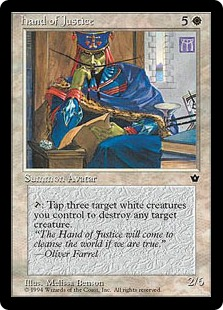
\includegraphics{hand}
		\end{center}

		Enquanto isso o elemental mistificando... amor [Se\c{c}\~ao \ref{amor}] puro \'e s\'o um dos atributos de $ \alpha_\omega $. \'E preciso consci\^encia para criar consci\^encias. ou n\~ao... Na verdade a consci\^encia de bem e mal s\'o existe a partir do homem. Animais fazem tudo por instinto, mas uma dem\^onia\cite{x} alegando que matou por instinto n\~ao \'e aceita. O ju\'izo de consci\^encia...

		\begin{center}
			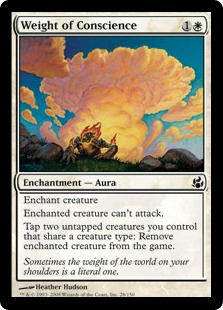
\includegraphics{conscience} 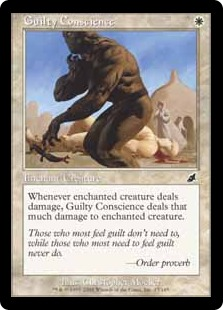
\includegraphics{guilty}

			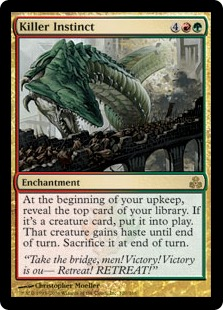
\includegraphics{killer} 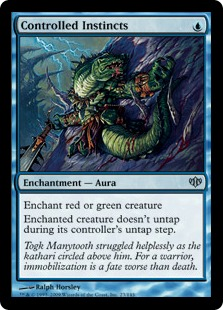
\includegraphics{controlled}
		\end{center}

		Ou \'e poss\'ivel p\^or l\'ogica na Vida, na psicologia, na espiritualidade, na moral, no amor. Ou algo transcende a l\'ogica.

		Existe como falar de aquecimento global sem terrorismo? Ciclones/furac\~oes no Brasil! Meteoros!

		\begin{flushright}
		\end{flushright}

		Como seria a g\^enese do bem e do mal? A m\^onada... Como seria a g\^enese das dimens\~oes? No princ\'ipio seja o ponto. Ap\'os uma transforma\c{c}\~ao qu\^antica, passou a existir uma reta. Da\'i ela se dividiu em duas, e houve o salto para a terceira dimens\~ao. Podemos conceber uma dimens\~ao e meia.

		Um ponto se moveu em 1D: $x = A $ sen $\omega t$.

		2D = pr\'oton e el\'etron. $\binom{x}{y} = A \binom{\cos \omega t}{\mbox{sen } \omega t}$.

		O magnetismo cria a necessidade da 3$^a$ dimens\~ao. $\mathbf{r} = (x,y,z) = \lambda \mathbf{u} + \mu \mathbf{v}; \mathbf{r}''(t) + A \omega^2 \mathbf{r} = 0$.

		Barbante do tempo. Suponhamos novamente que reencarnar \'e viajar no tempo. Num universo em que tudo \'e um, $\dim U = 0$. A partir do momento em que h\'a diferen\c{c}as, seja a Individualidade, torna-se necess\'ario no m\'inimo uma reta. $\dim U \ge 1$. E a partir do momento em que alguma coisa se move, existe a dimens\~ao temporal. (Tem isso na G\^enese, cace-se.) Como poderia ter o tempo dois graus de liberdade? Instante antes, instante depois, instante \`a direita, instante \`a esquerda, instante acima, instante abaixo.

		\begin{flushright}
		\end{flushright}

		Retroalimenta\c{c}\~ao: $E_a$ sem $E_c =$ disciplina. $E_c$ sem $E_a =$ semi-consci\^encia. Consequ\^encias morais da gravidade.

		\begin{flushright}
		\end{flushright}

		A lei do livre arb\'itrio. A lei do instinto. A lei do princ\'ipio inteligente versus o princ\'ipio espiritual versus o princ\'ipio vital...

	\section{Em que acredito}
			\begin{flushright}
			\end{flushright}

		\begin{center}
		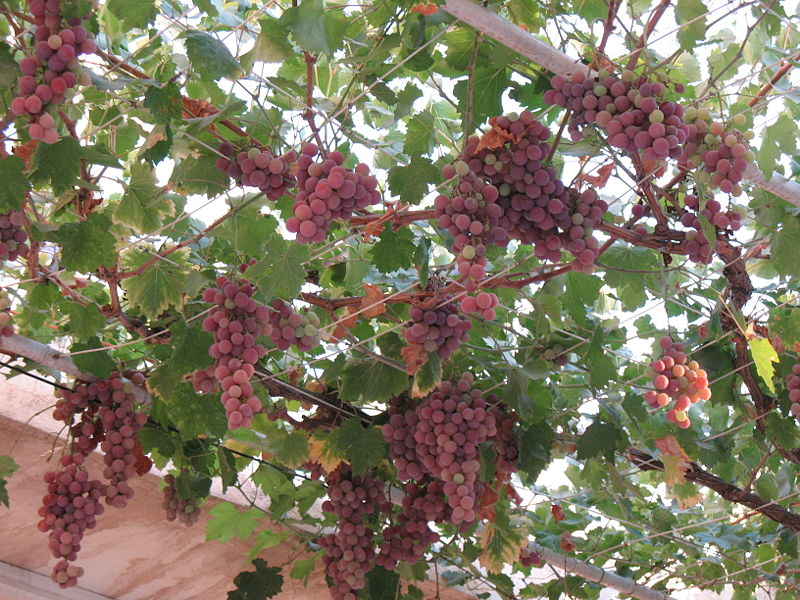
\includegraphics{vitis_vinifera}
		\end{center}

		\subsection{Verdades}
			\begin{flushright}
			\end{flushright}

			Veja a Se\c{c}\~ao \ref{verdade}.

			Redefini\c{c}\~oes:

			\begin{center}
				\begin{tabular}{|c|c|}
					\hline
					Verdade & Ilus\~ao \\
					\hline
					Amor [Se\c{c}\~ao \ref{amor}] & Sexo $ \Rightarrow $ Instinto $ \Rightarrow $ Mat\'eria \\
					Bem & Igreja\cite{igreja} \\
					Brama indiano, o n\~ao percebido & Maia indiano, o manifesto \\
					Consci\^encia & Ego \\
					Consequ\^encias &  \\
					$ \alpha_\omega $ & Demonismo\cite{demomono} \\
					Educa\c{c}\~ao da Alma & Autoridades religiosas \\
					Ess\^encia [Se\c{c}\~ao \ref{essencia}] & Dualidade \\
					Esp\'irito & Imperfei\c{c}\~oes \\
					Evolu\c{c}\~ao, Progresso & \\
					Igualdade [Se\c{c}\~ao \ref{leiIgualdade}] & Consumo \\
					Interno & Externo\\
					Justi\c{c}a [Se\c{c}\~ao \ref{escAxiomas}] & Caos \\
					Liberdade\cite{liberdade}, Perfei\c{c}\~ao [Se\c{c}\~ao \ref{serPerfeito}] & Finitude [Se\c{c}\~ao \ref{criaturaCriador}] \\
					Medita\c{c}\~ao & Pensamento \\
					Natureza & Sobrenatural \\
					Paranormalidade & Intermedi\'ario entre Criador e criatura \\
					Paz & Raiva\cite{bomCombate} $ \Rightarrow $ orgulho, ego\'ismo \\
					Prazer & Mal \\
					Reencarna\c{c}\~ao [Se\c{c}\~ao \ref{escAxiomas}] & Monoencarnacionismo\cite{demomono} \\
					Transcend\^encia & Dor \\
					Unidade \cite{unidade} & Desejo \cite{desejo} \\
					Vida & Morte \\
					Virtudes & Sangue \\
					\hline
				\end{tabular}
			\end{center}

			\subsubsection{Verdadeira caridade}
				\begin{flushright}
				\end{flushright}

                Benevol\^encia para com todos, indulg\^encia para as imperfei\c{c}\~oes [Se\c{c}\~ao \ref{serPerfeito}] dos outros, perd\~ao das ofensas. (\cite{le} q. 886)

				Elementos da verdadeira caridade: benevol\^encia, indulgencia, abnega\c{c}\~ao, devotamento (\cite{ese} cap. 17, item 2)

			\subsubsection{Verdadeira ci\^encia}
				\begin{flushright}
				\end{flushright}

				A ci\^encia pode estar cheia de poder, mas s\'o o amor [Se\c{c}\~ao \ref{amor}] beneficia. A ci\^encia, em todas as \'epocas, conseguiu in\'umeras express\~oes evolutivas. Vemo-la no mundo, exibindo realiza\c{c}\~oes que pareciam quase inating\'iveis. M\'aquinas enormes cruzam os ares e o fundo dos oceanos. A palavra \'e transmitida, sem fios, a longas dist\^ancias. A imprensa difunde racioc\'inios mundiais. Mas, para essa mesma ci\^encia pouco importa que o homem lhe use os frutos para o bem ou para o mal. N\~ao compreende o desinteresse, nem as finalidades santas.

				O amor, por\'em, aproxima-se de seus labores e retifica-os, conferindo-lhe a consci\^encia do bem. Ensina que cada m\'aquina deve servir como utilidade divina, no caminho dos homens para $ \alpha_\omega $, que somente se deveria transmitir a palavra edificante como d\'adiva do Alt\'issimo, que apenas seria justa a publica\c{c}\~ao dos racioc\'inios elevados para o esfor\c{c}o redentor das criaturas.

				Se a ci\^encia descobre explosivos, esclarece o amor quanto \`a utiliza\c{c}\~ao deles na abertura de estradas que liguem os povos; se a primeira confecciona um livro, ensina o segundo como gravar a verdade consoladora. A ci\^encia pode concretizar muitas obras \'uteis, mas s\'o o amor institui as obras mais altas. N\~ao duvidamos de que a primeira, bem interpretada, possa dotar o homem de um cora\c{c}\~ao corajoso; entretanto, somente o segundo pode dar um cora\c{c}\~ao iluminado.

				O mundo permanece em obscuridade e sofrimento, porque a ci\^encia foi assalariada pelo \'odio, que aniquila e perverte, e s\'o alcan\c{c}ar\'a o porto de seguran\c{c}a quando se render plenamente ao amor de Jesus-Cristo.

				\cite{cvv}, 152, Ci\^encia e Amor

			\subsubsection{Verdadeiro cil\'icio}
			\begin{flushright}
			\end{flushright}

				Se quereis um cil\'icio, aplicai-o \`as vossas almas e n\~ao aos vossos corpos; mortificai o vosso Esp\'irito e n\~ao a vossa carne; fustigai o vosso orgulho, recebei sem murmurar as humilha\c{c}\~oes; flagiciai o vosso amor-pr\'oprio; enrijai-vos contra a dor da inj\'uria e da cal\'unia, mais pungente do que a dor f\'isica. A\'i tendes o verdadeiro cil\'icio cujas feridas vos ser\~ao contadas, porque atestar\~ao a vossa coragem e a vossa submiss\~ao \`a vontade de $ \alpha_\omega $\footnotemark[2]. (\cite{ese} cap. 5, item 26)

				\footnotetext[2]{Lista de S\'imbolos na Se\c{c}\~ao \ref{simbolos}} %para a secao em que acredito

			\subsubsection{Verdadeira desgra\c{c}a}
			\begin{flushright}
			\end{flushright}

				est\'a nas consequ\^encias de um fato, mais do que no pr\'oprio fato. (\cite{ese} cap. 5, item 24)

			\subsubsection{Verdadeiro esc\^andalo}
			\begin{flushright}
			\end{flushright}

				\'E tudo o que resulta dos v\'icios e das imperfei\c{c}\~oes \cite{aperfeicoamento} humanas, toda rea\c{c}\~ao m\'a de um indiv\'iduo para outro, com ou sem repercuss\~ao. O esc\^andalo, neste caso, \emph{\'e o resultado efetivo do mal moral} [Se\c{c}\~ao \ref{amor}]. (\cite{ese} cap. 8, item 12)

			\subsubsection{Verdadeira f\'e}\label{feh}
				\begin{flushright}
				\end{flushright}

				\emph{F\'e inabal\'avel s\'o o \'e a que pode encarar de frente a raz\~ao, em todas as \'epocas da Humanidade.} (\cite{ese} cap. 19, item 7)

				A f\'e sincera e verdadeira \'e sempre calma; faculta a paci\^encia que sabe esperar, porque, tendo seu ponto de apoio na intelig\^encia e na compreens\~ao das coisas, tem a certeza de chegar ao objetivo visado. (\cite{ese} cap. 19, item 3)

				Acrescentando: \textquotedblleft Tua f\'e te salvou\textquotedblright, fez ver que $ \alpha_\omega $ considera o que h\'a no \^amago do cora\c{c}\~ao e n\~ao a forma exterior da adora\c{c}\~ao. (...) Dizendo ao samaritano: \textquotedblleft Tua f\'e te salvou\textquotedblright, d\'a Jesus a entender que o mesmo n\~ao aconteceu aos outros. (\cite{genese} cap. 15, item 17)

			\subsubsection{Verdadeira for\c{c}a}
			\begin{flushright}
			\end{flushright}

				II Cor\'intios 12, 10.

			\subsubsection{Verdadeiro homem}\label{homem}
				\begin{flushright}
				\end{flushright}

				\textquotedblleft...Eis o Homem!\textquotedblright\, | Pilatos. (Jo\~ao 19, 5)

				Apresentando o Cristo \`a multid\~ao, Pilatos n\~ao designava um triunfador terrestre...

				Nem banquete, nem p\'urpura.

				Nem aplauso, nem flores.

				Jesus achava-se diante da morte.

				Terminava uma semana de terr\'iveis flagela\c{c}\~oes\cite{autoflagelo}.

				Tra\'ido, n\~ao se rebelara.

				Preso, exercera a paci\^encia.

				Humilhado, n\~ao se entregou a revides.

				Esquecido, n\~ao se confiou \`a revolta.

				Escarnecido, desculpara.

				A\c{c}oitado, olvidou a ofensa.

				Injusti\c{c}ado, n\~ao se defendeu.

				Sentenciado ao mart\'irio, soube perdoar.

				Crucificado, voltaria \`a conviv\^encia dos mesmos disc\'ipulos e benefici\'arios que o haviam abandonado, para soerguer-lhes a esperan\c{c}a.

				Mas, exibindo-o, diante do povo, Pilatos n\~ao afirma: | Eis o condenado, eis a v\'itima!

				Diz simplesmente: | \textquotedblleft Eis o Homem!\textquotedblright

				Aparentemente vencido, o Mestre surgia em plena grandeza espiritual, revelando o mais alto padr\~ao de dignidade humana.

				Rememorando, pois, semelhante passagem, recordemos que somente nas linhas morais [Se\c{c}\~ao \ref{amor}] do Cristo \'e que atingiremos a Humanidade Real.

				\cite{fonteViva}, 127, Humanidade Real

			\subsubsection{Verdadeira igreja}
			\begin{flushright}
			\end{flushright}

                        \cite{igreja}

			\subsubsection{Verdadeira igualdade / Lei de igualdade}\label{leiIgualdade}
			\begin{flushright}
			\end{flushright}

				A mulher formada de uma costela de Ad\~ao \'e uma alegoria, aparentemente pueril, se admitida ao p\'e da letra, mas profunda, quanto ao sentido. Tem por fim mostrar que a mulher \'e da mesma natureza que o homem, que \'e por conseguinte igual a este perante $ \alpha_\omega $ e n\~ao uma criatura \cite{criatura} \`a parte, feita para ser escravizada e tratada qual hilota. Tendo-a como sa\'ida da pr\'opria carne do homem, a imagem da igualdade \'e bem mais expressiva, do que se ela fora tida como formada, separadamente, do mesmo limo. Equivale a dizer ao homem que ela \'e sua igual e n\~ao sua escrava, que ele a deve amar como parte de si mesmo. (\cite{genese}, cap. 12, item 11)

			\subsubsection{Verdadeiro prazer}
			\begin{flushright}
			\end{flushright}

				Se unicamente busc\'asseis a vol\'upia que uma a\c{c}\~ao boa proporciona, conservar-vos-\'ieis sempre na senda do progresso [Se\c{c}\~ao \ref{serPerfeito}] espiritual. (\cite{ese}, cap. 13, item 12)

			\subsubsection{Verdadeira propriedade}
			\begin{flushright}
			\end{flushright}

				aquilo que nos \'e dado levar deste mundo. Tudo o que \'e de uso da alma: a intelig\^encia, os conhecimentos, as qualidades morais [Se\c{c}\~ao \ref{amor}]. (\cite{ese}, cap. 16, item 9)

  			Riqueza \'e ilus\~ao\cite{ilusao}. Mateus 13, 18-23 (\cite{ese}, cap. 17, itens 5-6)

			\subsubsection{Verdadeira pureza}
				\begin{flushright}
				\end{flushright}

				n\~ao est\'a somente nos atos; est\'a tamb\'em no pensamento. (\cite{ese}, cap. 8, item 6)

				Mateus 15, 18-19 \cite{palavras}.
				Os judeus haviam desprezado os verdadeiros mandamentos de $ \alpha_\omega $ para se aferrarem \`a pr\'atica dos regulamentos que os homens tinham estatu\'ido e da r\'igida observ\^ancia desses regulamentos faziam casos de consci\^encia [Se\c{c}\~ao \ref{amor}]. A subst\^ancia, muito simples, acabara por desaparecer debaixo da complica\c{c}\~ao da forma. Como fosse muito mais f\'acil praticar atos exteriores, do que se reformar moralmente, \emph{lavar as m\~aos do que expurgar o cora\c{c}\~ao}, iludiram-se a si pr\'oprios os homens, tendo-se como quites para com $ \alpha_\omega $, por se conformarem com aquelas pr\'aticas, conservando-se tais quais eram, visto se lhes ter ensinado que $ \alpha_\omega $ n\~ao exigia mais do que isso. Dai o haver dito o profeta: \emph{\'E em v\~ao que este povo me honra de l\'abios, ensinando m\'aximas e ordena\c{c}\~oes humanas.}

				Verificou-se o mesmo com a doutrina moral [Se\c{c}\~ao \ref{amor}] do Cristo, que acabou por ser atirada para segundo plano, donde resulta que muitos crist\~aos, a exemplo dos antigos judeus, consideram mais garantida a salva\c{c}\~ao \cite{salvacao} por meio das pr\'aticas exteriores, do que pelas da moral. E a essas adi\c{c}\~oes, feitas pelos homens \`a lei de $ \alpha_\omega $, que Jesus alude, quando diz: \emph{Arrancada ser\'a toda planta que meu Pai celestial n\~ao plantou.}

				O objetivo da religi\~ao \'e conduzir a $ \alpha_\omega $ o homem [Se\c{c}\~ao \ref{homem}]. Ora, este n\~ao chega a $ \alpha_\omega $ sen\~ao quando se torna perfeito [Se\c{c}\~ao \ref{serPerfeito}]. Logo, toda religi\~ao que n\~ao torna melhor o homem, n\~ao alcan\c{c}a o seu objetivo. Toda aquela em que o homem julgue poder apoiar-se para fazer o mal, ou \'e falsa, ou est\'a falseada em seu princ\'ipio. Tal o resultado que d\~ao as em que a forma sobreleva ao fundo. Nula \'e a cren\c{c}a na efic\'acia dos sinais exteriores, se n\~ao obsta a que se cometam assass\'inios, adult\'erios, espolia\c{c}\~oes, que se levantem cal\'unias, que se causem danos ao pr\'oximo, seja no que for. Semelhantes religi\~oes fazem supersticiosos, hip\'ocritas, fan\'aticos; n\~ao, por\'em, homens de bem.

				N\~ao basta se tenham as apar\^encias da pureza; acima de tudo, \'e preciso ter a do cora\c{c}\~ao. (\cite{ese}, cap. 8, item 10)

		\subsection{\href{http://sites.google.com/site/mathspirituality/portugues/PaiNosso.ASF?attredirects=0}{Pai Nosso}}\label{PaiNosso}
			\begin{flushright}
			\end{flushright}

			Pai de Infinito Amor [Se\c{c}\~ao \ref{amor}], que estais dentro [Se\c{c}\~ao \ref{serPerfeito}] e fora de n\'os,

			santifiquemo-nos e santificado ser\'a o vosso nome.

			Aproximai-nos de nossa Verdadeira Natureza.

			Seja feita vossa vontade, tanto na personalidade quanto na individualidade [Se\c{c}\~ao \ref{leiPerfeicao}].

			Dai-nos hoje o p\~ao sobressubstancial.

			Perdoai-nos nossas d\'ividas,

			assim como j\'a perdoamos aos nossos devedores.

			N\~ao nos induzais a novas prova\c{c}\~oes.

			Mas libertai-nos da mat\'eria.

			Porque s\'o vosso \'e o reino, o poder, a honra e a gl\'oria por toda a eternidade.

			Assim seja.

			\begin{flushright}
			\end{flushright}

			\textquotedblleft E Jesus, vendo a multid\~ao\cite{perseguicao}, subiu a um monte...\textquotedblright\, | (Mateus 5, 1)

			O procedimento dos homens cultos para com o povo experimentar\'a eleva\c{c}\~ao crescente \`a medida que o Evangelho se estenda nos cora\c{c}\~oes.

			Infelizmente, at\'e agora, raramente a multid\~ao tem encontrado, por parte das grandes personalidades humanas, o tratamento a que faz jus.

			Muitos sobem ao monte da autoridade e da fortuna, da intelig\^encia e do poder, mas simplesmente para humilh\'a-la ou esquec\^e-la depois.

			Sacerdotes in\'umeros enriquecem-se de saber e buscam subjug\'a-la a seu talante.

			Pol\'iticos astuciosos exploram-lhe as paix\~oes em proveito pr\'oprio.

			Tiranos disfar\c{c}ados em condutores envenenam-lhe a alma e arrojam-na ao despenhadeiro da destrui\c{c}\~ao, \`a maneira dos algozes de rebanho que apartam as reses para o matadouro.

			Ju\'izes menos preparados para a dignidade das fun\c{c}\~oes que exercem, confundem-lhe o racioc\'inio.

			Administradores menos escrupulosos arregimentam-lhe as express\~oes num\'ericas para a cria\c{c}\~ao de efeitos contr\'arios ao progresso.

			Em todos os tempos, vemos o trabalho dos leg\'itimos mission\'arios do bem prejudicado pela ignor\^ancia que estabelece perturba\c{c}\~oes e espantalhos para a massa popular.

			Entretanto, para a comunidade dos aprendizes do Evangelho, em qualquer clima da f\'e [Se\c{c}\~ao \ref{feh}], o padr\~ao de Jesus brilha soberano.

			Vendo a multid\~ao, o Mestre sobe a um monte e come\c{c}a a ensinar...

			\'E imprescind\'ivel empenhar as nossas energias, a servi\c{c}o da educa\c{c}\~ao.

			Ajudemos o povo a pensar, a crescer e a aprimorar-se\cite{aperfeicoamento}.

			Auxiliar a todos para que todos se beneficiem e se elevem, tanto quanto n\'os desejamos melhoria e prosperidade para n\'os mesmos, constitui para n\'os a felicidade real e indiscut\'ivel.

			Ao leste e ao oeste, ao norte e ao sul da nossa individualidade, movimentam-se milhares de criaturas, em posi\c{c}\~ao inferior \`a nossa.

			Estendamos os bra\c{c}os, alonguemos o cora\c{c}\~ao e irradiemos entendimento, fraternidade e simpatia, ajudando-as sem condi\c{c}\~oes.

			Quando o crist\~ao pronuncia as sagradas palavras \textquotedblleft Pai Nosso\textquotedblright, est\'a reconhecendo n\~ao somente a Paternidade de $ \alpha_\omega $, mas aceitando tamb\'em por sua fam\'ilia a Humanidade inteira.

		\subsection{Apocalipse}
			\begin{flushright}
			\end{flushright}

			Veja \cite{apocalipse}.

		\subsection{Lei de amor e caridade}
			\begin{flushright}
			\end{flushright}

			Mateus\cite{palavrasAtiradas} 5, 21-22.

			Jesus faz da brandura, da modera\c{c}\~ao, da mansuetude, da afabilidade e da paci\^encia, uma lei. Condena, por conseguinte, a viol\^encia, a c\'olera e at\'e toda express\~ao descort\^es de que algu\'em possa usar para com seus semelhantes. \emph{Raca}, entre os hebreus, era um termo desdenhoso que significava | \emph{homem que n\~ao vale nada}, e se pronunciava cuspindo e virando para o lado a cabe\c{c}a. Vai mesmo mais longe, pois que amea\c{c}a com o fogo do inferno\cite{demonismo} aquele que disser ao seu irm\~ao: \emph{\'Es louco\cite{mistificacao}.}

			Evidente se torna que aqui, como em todas as circunst\^ancias, a inten\c{c}\~ao agrava ou atenua a falta; mas, em que pode uma simples palavra revestir-se de tanta gravidade que mere\c{c}a t\~ao severa reprova\c{c}\~ao? \'E que toda a palavra ofensiva\cite{palavrasAtiradas} exprime um sentimento contr\'ario \`a lei do amor e da caridade [Se\c{c}\~ao \ref{amor}] que deve presidir \`as rela\c{c}\~oes entre os homens e manter entre eles a conc\'ordia e a uni\~ao\cite{unidade}; \'e que constitui um golpe desferido na benevol\^encia rec\'iproca e na fraternidade; \'e que entret\'em o \'odio e a animosidade; \'e, enfim, que, depois da humildade para com $ \alpha_\omega $, a caridade para com o pr\'oximo \'e a lei primeira de todo crist\~ao. (\cite{ese}, cap. 9, item 4)

	\section{F\'isica $ \times $ Materialismo}\label{fisica}
		\begin{flushright}
		\end{flushright}

		O esp\'irito precisa da mat\'eria, que precisa do esp\'irito. Mas que mat\'eria \'e essa? Antimat\'eria, mat\'eria escura... \'E mais absurdo um h\'adron ou um esp\'irito?

		\begin{center}
			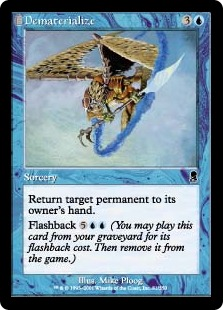
\includegraphics{dematerialize} 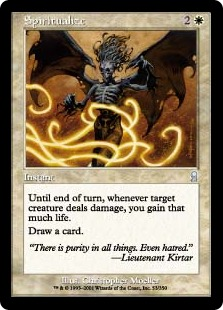
\includegraphics{spiritualize}

			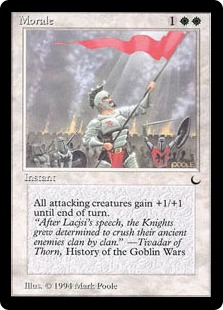
\includegraphics{morale} 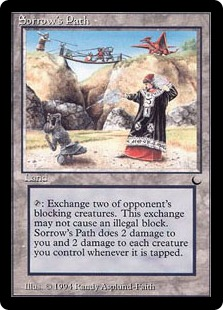
\includegraphics{sorrow}

			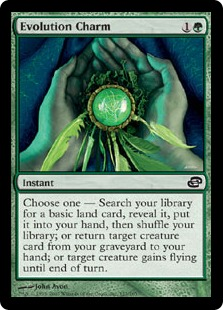
\includegraphics{charm} 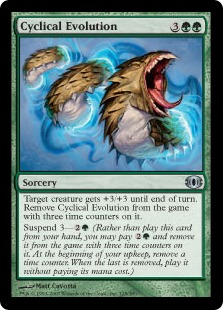
\includegraphics{cyclical}

			\includegraphics{parallel} 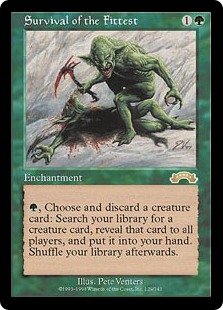
\includegraphics{survival}

			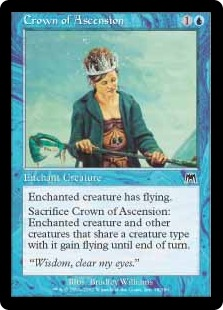
\includegraphics{ascension}
		\end{center}

		Em Planck\cite{planck}, um el\'etron se teletransporta.

		Para eu teletransportar o objeto $x$ da posi\c{c}\~ao $\mathbf{r}_1$ a $\mathbf{r}_2$, n\~ao basta saber tudo sobre $x$. \'E preciso saber tudo de $r_1$ a $r_2$, para alterar as informa\c{c}\~oes de $r_1$ e $r_2$.

		Existe caminho cont\'inuo [Se\c{c}\~ao \ref{continuidade}] de $\mathbf{r}_1$ a $\mathbf{r}_2$, passando por outros Universos? Para algum caminho, dist$(\mathbf{r}_1, \mathbf{r}_2) = \delta $.

	\section{Tecnologia da Informa\c{c}\~ao}
			\begin{flushright}
			\end{flushright}

		\subsection{Relat\'orio T\'ecnico Final (CEFET-MG)}
			\begin{flushright}
			\end{flushright}

			\href{https://github.com/boralaemcasa/propagation/tree/master/webs%20dot%20com/info/reltec.pdf}{PDF}

			Pacote ZIP \href{https://github.com/boralaemcasa/propagation/tree/master/webs%20dot%20com/info/reltec.zip}{Completo}

		\subsection{\emph{Software} Livre em \emph{Object Pascal}}
			\begin{flushright}
			\end{flushright}

			\href{https://github.com/boralaemcasa/propagation/tree/master/webs%20dot%20com/info/cubo.zip}{Cubo} | V\^em embutidas as fun\c{c}\~oes PontoXY e PontoXYZ para plotar pontos em coordenadas 2D e 3D.

			Grandes Primos \cite{primos}

			\href{https://github.com/boralaemcasa/propagation/tree/master/webs%20dot%20com/info/display.zip}{\emph{Display}} de 7 Segmentos

			\subsubsection{Strings Num\'ericas}
				\begin{flushright}
				\end{flushright}

				Fazer contas em $ \mathbb{Q} $ \footnotemark[1] sem limite?

				\footnotetext[1]{Lista de S\'imbolos na Se\c{c}\~ao \ref{simbolos}} %para a secao informatica

				\scriptsize
				\begin{verbatim}

unit SNum;

interface

const
   PRIMOS_SOURCE = 'D:\Matemática\primos novos.dat';
   // Download from http://sites.google.com/site/mathspirituality/Home/newprimes.part01.rar?attredirects=0
   //               http://sites.google.com/site/mathspirituality/Home/newprimes.part02.rar?attredirects=0

var
   PRIMO_LIMITE: longword;

type
   SFrac = record
      n, d: string;
   end;

   function Valida(s: string): string;

// as funçoes abaixo já partem de que as strings sao válidas
   function  Soma(a,b: string): string;
   function  Subtrai(a,b: string): string;
   function  Multiplica(a,b: string): string;
   procedure Divide(a,b: string; var q,r: string);
   function  Potencia(a,b: string): string;

   function  SNumCompare(a,b: string): shortint;
   function  Oposto(s: string): string;

   function  FatoresPrimos(x: string): string;

// fraçoes
   function  Str2SFrac(a: string; b: string = ''): SFrac;
   procedure SFracReduz(var frac: SFrac);
   function  SFracDizima(frac: SFrac): string;

   function  SFracAdd(a, b: SFrac): SFrac;
   function  SFracSub(a, b: SFrac): SFrac;
   function  SFracMul(a, b: SFrac): SFrac;
   function  SFracDiv(a, b: SFrac): SFrac;

implementation

uses SysUtils, Forms;

procedure ZeroLTrim(var s: string);
begin
  while (copy(s, 1, 1) = '0') and (length(s) > 1) do
    delete(s, 1, 1);
end;

function Valida(s: string): string;
var i: integer;
begin
   i := 1;
   if s = '' then s := '0';
   if s[1] = '-' then inc(i);
   while i <= length(s) do
      begin
         if s[i] in ['0'..'9']
            then inc(i)
            else delete(s, i, 1);
      end;

   Result := s;
   ZeroLTrim(Result);
end;

function  Soma(a,b: string): string;
var i, x: integer;
    carry: byte;
    minus: boolean;
begin
  minus := false;
  if copy(a, 1, 1) = '-' then
     begin
        delete(a, 1, 1);
        if copy(b, 1, 1) = '-' then
           begin
              delete(b, 1, 1);
           // -a + (-b) = -(a + b)
              minus := true;
           end
        else
           begin
           // -a + b = b - a
              Result := Subtrai(b, a);
              exit;
           end;
     end
  else if copy(b, 1, 1) = '-' then
     begin
        delete(b, 1, 1);
     // a + (-b) = a - b
        Result := Subtrai(a, b);
        exit;
     end;

  if length(a) > length(b) then // troca a, b
  begin
    Result := a;
    a := b;
    b := Result;
  end;

  x := length(b);
  while length(a) < x do
    a := '0' + a;

//008765
//123400
  i := x;
  while (i > 0) and (b[i] = '0') do
    dec(i);

  Result := copy(a, i + 1, x - i);
  delete(a, i + 1, x - i);
  delete(b, i + 1, x - i);

  carry := 0;
  for i := i downto 1 do
     begin
        x := byte(a[i]) - 48 + byte(b[i]) - 48 + carry;
        if x >= 10 then
           begin
              carry := 1;
              dec(x, 10);
           end
        else carry := 0;
        Result := char(x + 48) + Result;
     end;
  if carry <> 0 then
     Result := '1' + Result;
  if minus then
     Result := '-' + Result;
end;

function  Subtrai(a,b: string): string;
var i: integer;
    x, carry: shortint;
begin
   if copy(a, 1, 1) = '-' then
      begin
         delete(a, 1, 1);
         if copy(b, 1, 1) = '-' then
            begin
               delete(b, 1, 1);
            // -a - (-b) = b - a
               Result := Subtrai(b, a);
            end
         else
            begin
            // -a - b = -(a + b)
               Result := '-' + Soma(a, b);
            end;
         exit;
      end
   else if copy(b, 1, 1) = '-' then
      begin
         delete(b, 1, 1);
      // a - (-b) = a + b
         Result := Soma(a, b);
         exit;
      end
   else if SNumCompare(a, b) < 0 then
      begin
      // a < b => a - b = -(b - a)
         Result := '-' + Subtrai(b, a);
         exit;
      end;
// 923
// 199
   while length(b) < length(a) do
      b := '0' + b;
   Result := '';
   carry := 0;
   for i := length(a) downto 1 do
      begin
         x := byte(a[i]) - 48 - byte(b[i]) + 48 - carry;
         if x < 0 then
            begin
               carry := 1;
               inc(x, 10);
            end
         else carry := 0;
         Result := char(x + 48) + Result;
      end;

  ZeroLTrim(Result);
end;

function  SNumCompare(a,b: string): shortint;
var minus: boolean;
begin
   Result := 0;
   if a = b then exit;
   minus := false;
   if copy(a, 1, 1) = '-' then
      if copy(b, 1, 1) = '-'
         then minus := true
         else Result := -1
   else if copy(b, 1, 1) = '-' then
      Result := -1;

   if Result <> 0 then exit;

   if minus then
      begin
         delete(a, 1, 1);
         delete(b, 1, 1);
      end;

   while length(b) < length(a) do
      b := '0' + b;
   while length(a) < length(b) do
      a := '0' + a;

// positivos
   if a > b
      then Result := 1
      else Result := -1;

// negativos inverte
   if minus then Result := - Result;
end;

function  Multiplica(a,b: string): string;
var i, j: integer;
    x, carry: byte;
    minus: boolean;
    subtotal: string;
    multAlgarismo: array[2..9] of string;
begin
   minus := (copy(a, 1, 1) = '-');
   if minus then delete(a, 1, 1);
   if copy(b, 1, 1) = '-' then
      begin
         delete(b, 1, 1);
         minus := not minus;
      end;

   for i := 2 to 9 do
   begin
     multAlgarismo[i] := '';
     carry := 0;

  // multiplicar i por cada algarismo de a
     for j := length(a) downto 1 do
        begin
           x := (byte(a[j]) - 48) * i + carry;
           carry := x div 10;
           x := x mod 10;
           multAlgarismo[i] := char(x + 48) + multAlgarismo[i];
        end;

     if carry <> 0 then
        multAlgarismo[i] := char(carry + 48) + multAlgarismo[i];
   end;

   Result := '0';
   for i := length(b) downto 1 do
     if b[i] <> '0' then
       begin
         subtotal := '';
      // zeros aa direita
         if i < length(b) then
            for j := 1 to length(b) - i do
               subtotal := '0' + subtotal;

         if b[i] = '1'
           then subtotal := a + subtotal
           else subtotal := multAlgarismo[(byte(b[i]) - 48)] + subtotal;

      // o resultado é a soma dos subtotais
         Result := soma(Result, subtotal);
       end;

   ZeroLTrim(Result);

   if minus then
      Result := '-' + Result;
end;

procedure Divide(a,b: string; var q,r: string);
var minusa, minusb: boolean;
    x: byte;
    index: integer;
begin
   if b = '0' then
      begin
         q := '0';
         r := '0';
         exit;
      end;

   minusa := (copy(a, 1, 1) = '-');
   minusb := (copy(b, 1, 1) = '-');
   if minusa then delete(a, 1, 1);
   if minusb then delete(b, 1, 1);

   q := '';
   index := length(b);
   r := copy(a, 1, index);
   repeat
      x := 0;
      while SNumCompare(r, b) >= 0 do
         begin
            inc(x);
            r := Subtrai(r, b);
         end;
      q := q + char(x + 48);
      if index >= length(a) then break;

   // "baixar" o próximo
      inc(index);
      if r = '0' then r := ''; // zero de resto nao vai virar zero aa esq
      r := r + a[index];
   until false;

   ZeroLTrim(q);

//  7 /  4 = ( 1, 3)     a < 0, r > 0:  incrementar o módulo do quociente
// -7 /  4 = (-2, 1)                   complementar o resto
//  7 / -4 = (-1, 3)     exatamente um negativo: sinal '-' no quociente
// -7 / -4 = ( 2, 1)
   if minusa and (r <> '0') then
      begin
         q := Soma(q, '1');
         r := Subtrai(b, r);
      end;
   if minusa xor minusb then
      q := '-' + q;
end;

function  Oposto(s: string): string;
begin
   if copy(s, 1, 1) = '-'
      then delete(s, 1, 1)
      else insert('-', s, 1);

   Result := s;
end;

function Potencia(a,b: string): string;
begin
  if SNumCompare(b, '0') <= 0 then
    Result := '1'
  else begin
    Result := a;
    while b <> '1' do
    begin
      Result := Multiplica(result, a);
      b := Subtrai(b, '1');
    end
  end;
end;

function Str2SFrac(a: string; b: string = ''): SFrac;
begin
   if b = '' then b := '1';
   Result.n := a;
   Result.d := b;
end;

function SFracAdd(a, b: SFrac): SFrac;
//var c: SFrac;
//    mdc, q1, q2, r: string;
begin
{
// reduzir a fraçao com os 2 denominadores => c
   c.n := a.d;
   c.d := b.d;
   SFracReduz(c);
   Divide(b.d, c.d, mdc, r);
   Divide(Multiplica(a.n, b.d), mdc, q1, r);
   Divide(Multiplica(a.d, b.n), mdc, q2, r);
   Result.n := Soma(q1, q2);
   Divide(Multiplica(a.d, b.d), mdc, q1, r);
   Result.d := q1;
   SFracReduz(Result);
}
   Result.n := Soma(Multiplica(a.n, b.d), Multiplica(a.d, b.n));
   Result.d := Multiplica(a.d, b.d);
   SFracReduz(Result);
end;

function SFracSub(a, b: SFrac): SFrac;
begin
   b.n := Oposto(b.n);
   Result := SFracAdd(a, b);
{
   Result.n := Subtrai(Multiplica(a.n, b.d), Multiplica(a.d, b.n));
   Result.d := Multiplica(a.d, b.d);
   SFracReduz(Result);
}
end;

function SFracMul(a, b: SFrac): SFrac;
//var aux: string;
begin
{
   aux := b.d;
   b.d := a.d;
   a.d := aux;
   SFracReduz(a);
   SFracReduz(b);
   Result.n := Multiplica(a.n, b.n);
   Result.d := Multiplica(a.d, b.d);
}
   Result.n := Multiplica(a.n, b.n);
   Result.d := Multiplica(a.d, b.d);
   SFracReduz(Result);
end;

function SFracDiv(a, b: SFrac): SFrac;
var aux: string;
begin
   aux := b.n;
   b.n := b.d;
   b.d := aux;
   Result := SFracMul(a, b);
end;

procedure SFracReduz(var frac: SFrac);
var f: file of longword;
    p: longword;
    ps, x, y, q1, q2, r: string;
    minusn, minusd,
    divx, divy: boolean;
begin
   FileMode := 0; // read only
   AssignFile(f, PRIMOS_SOURCE);
   reset(f);

   minusn := (copy(frac.n, 1, 1) = '-');
   minusd := (copy(frac.d, 1, 1) = '-');
   if minusn then delete(frac.n, 1, 1);
   if minusd then delete(frac.d, 1, 1);
   if frac.n = '0' then frac.d := '1';

   x := frac.n;
   y := frac.d;
   p := 2;
   ps := '2';
   repeat //exercício: divisões sucessivas de Euclides ==> MDC
      Divide(x, ps, q1, r);
      divx := r = '0';
      Divide(y, ps, q2, r);
      divy := r = '0';

      if divx then x := q1;
      if divy then y := q2;
      if divx and divy then
         begin
            Divide(frac.n, ps, frac.n, r);
            Divide(frac.d, ps, frac.d, r);
         end;

      if not divx and not divy then
         begin
            read(f, p);
            ps := IntToStr(p);
         end;

      if (SNumCompare(x, ps) > 0) and (SNumCompare(x, IntToStr(p * p)) < 0) then
         ps := x
      else if (SNumCompare(y, ps) > 0) and (SNumCompare(y, IntToStr(p * p)) < 0) then
         ps := y;
   until (x = '1') or (y = '1') or eof(f) or (p > PRIMO_LIMITE);

   if (minusn xor minusd) and (frac.n <> '0') then
      frac.n := '-' + frac.n;

   CloseFile(f);
end;

function SFracDizima(frac: SFrac): string;
var d,           // dividendo
    alg,         // algarismo quociente
    restos: string;
    i, posicao: integer;
begin
   Divide(frac.n, frac.d, result, d);
   result := result + ',';
   restos := '.'; // é preciso ser entre pontos pq senao pega pedaço (4 de 14 p.ex.)
   posicao := 0; // só p/ nao dar warning

// achar o resto que se repete
{  exemplo:
       1/7 = (0,1)
      10/7 = 1,3
      30/7 = 4,2
      20/7 = 2,6
      60/7 = 8,4
      40/7 = 5,5
      50/7 = 7,1
      logo 1/7 = 0,(142857)
}
   if d <> '0' then
      repeat
         restos := restos + d + '.';      //.1.3.2.6.4.5.
         d := d + '0';
         Divide(d, frac.d, alg, d);
         result := result + alg;            //142857
         posicao := pos('.' + d + '.', restos);
      until (posicao > 0) or (d = '0');

   if d <> '0' then
      begin
      // contar os '.' da posiçao em diante (nro de algs da dízima)
         delete(restos, 1, posicao);
         posicao := 0;
         for i := 1 to length(restos) do
            if restos[i] = '.' then
               inc(posicao);

         insert('(', result, length(result) - posicao + 1);
         result := result + ')';
      end;
end;

function FatoresPrimos(x: string): string;
var fatorado, ps, q, r: string;
    f: file of longword;
    p: longword;
    expo: integer;
{
var x, ps, q, r, fatorado: string;
    p, p2: int64;
    n, counter, expo: integer;
}
begin
   if SNumCompare(x, '2') < 0 then
      begin
         Result := x;
         exit;
      end;

   fatorado := '';
   AssignFile(f, PRIMOS_SOURCE);
   reset(f);

   p := 2;
   ps := IntToStr(p);
   expo := 1;

   repeat
      Divide(x, ps, q, r);
      if (r = '0') and (x <> '0') then
         begin
            if pos(ps + ' * ', fatorado) > 0 then
               begin
                  inc(expo);
                  if q = '1' then
                     begin
                        fatorado := copy(fatorado, 1, length(fatorado) - 3);
                        fatorado := fatorado + ' ^ ' + IntToStr(expo) + ' * ';
                     end
               end
            else if expo = 1 then
               fatorado := fatorado + ps + ' * '
            else
               begin
                  fatorado := copy(fatorado, 1, length(fatorado) - 3);
                  fatorado := fatorado + ' ^ ' + IntToStr(expo) + ' * ' + ps + ' * ';
                  expo := 1;
               end;

            x := q;
         end
      else
      // próximo primo
         if eof(f) or (p > PRIMO_LIMITE) then
            ps := x
         else
            begin
               read(f, p);
               ps := inttostr(p);
            end;

      if (SNumCompare(x, ps) > 0) and (SNumCompare(x, Multiplica(ps, ps)) < 0) then
         ps := x;
   until x = '1';

   CloseFile(f);

   Result := copy(fatorado, 1, length(fatorado) - 3);
end;

begin
   PRIMO_LIMITE := 90000000;
end.
\end{verbatim}
				\normalsize

		\subsection{Exerc\'icio: Projeto S.I.A. | Sugest\~oes da Intelig\^encia Artificial}
			\begin{flushright}
			\end{flushright}

			O programa deve dialogar com o usu\'ario, como um BOT de IRC, e usar de psicologia centrada no cliente.
			Se o usu\'ario informar que gostaria de almo\c{c}ar, sugerir pratos e onde comer. Da mesma forma para qualquer tipo de consumo \cite{capital}.
			Ao informar que deseja fazer uma faculdade, mas n\~ao sabe qual, o sistema deve ter um m\'odulo vocacional.
			Informando que deseja saber alguma coisa, o sistema direciona para sua parte de enciclop\'edia interativa.
			Se o usu\'ario deseja ser alguma coisa construtiva, ent\~ao o sistema ajud\'a-lo-\'a. Caso seja alguma coisa negativa, o sistema ter\'a argumentos contra suas ideias.
			E se o ser n\~ao quiser nada, o sistema estimul\'a-lo-\'a a se autodescobrir.
			Deve ser previsto e evitado o caso de as pessoas ficarem dependentes de sugest\~oes do sistema.

    \subsection{Pedagogia $\times$ Rob\'otica}
		\begin{flushright}
		\end{flushright}

			\textquotedblleft rob\^o com sentimento\textquotedblright\, em ess\^encia \'e imposs\'ivel. Parece imposs\'ivel emular a alma.

			Qualquer programa, qualquer aproxima\c{c}\~ao de 99\% do sentimento humano, vai
 ser uma representa\c{c}\~ao, um ator. O ator representa um sentimento. \'E poss\'ivel sim um rob\^o que tem uma
personalidade pr\'e definida, ainda que variando no tempo.

Existe uma linha psicol\'ogica que diz que a gente aprende a \textquotedblleft sentir\textquotedblright\, da
mesma forma que nossas refer\^encias (os pais, av\'os, etc etc etc). Logo, \'e um processo pedag\'ogico. Um rob\^o que aprende a sentir?

    \subsection{Exerc\'icio: piloto autom\'atico do GPS de autom\'oveis e caminh\~oes}
		\begin{flushright}
		\end{flushright}

Detectar tudo: o sem\'aforo, os carros ao redor, a vaca, o pedestre, o poste, a
\'arvore caiu na frente. Pronto. Podemos eliminar todos os motoristas. Inclusive de ambul\^ancia. Preveja.

    \subsection{Conex\~ao N\~ao Local}
		\begin{flushright}
		\end{flushright}

 			Existe uma fronteira entre ciencia da computa\c{c}\~ao e fisica qu\^antica. Sup\~oem que o el\'etron \'e uma informa\c{c}\~ao. Isso me p\~oe para pensar na Informa\c{c}\~ao$(s)$.

    \subsection{Or\'aculo | Cliente Servidor}
		\begin{flushright}
		\end{flushright}

A ci\^encia \'e capaz de definir como vamos proceder? N\~ao. isso s\~ao
conven\c{c}\~oes sociais. No m\'aximo, a ci\^encia \'e capaz de construir um
supercomputador para o qual perguntamos: quais as consequ\^encias de
adotar um socialismo? uma teocracia?

Ele responde: de acordo com a an\'alise de todas as vari\'aveis poss\'iveis e
imagin\'aveis, a ado\c{c}\~ao tem 90\% de probabilidades de levar a sociedade e a
 humanidade para um buraco com caracter\'isticas $x, y$ e $z$. Voc\^es v\~ao
correr o risco? sim/n\~ao/cancelar

Da\'i as conven\c{c}\~oes adotadas podem ser, por exemplo, leis. A lei
anti-bingos n\~ao pegou...

Parece que nem as leis de Einstein, nem f\'isica qu\^antica, pegaram! T\^em
sim, consequencias sociais, n\~ao adotadas. No outro caso, \'e a pol\'icia brasileira que recebe ordens de bosta. E nesse caso, por que cargas d'\'agua n\~ao adotaram nem as consequ\^encias darwinianas?

		\begin{flushright}
		\end{flushright}

		\begin{verbatim}
in principio erat verbum...
\end{verbatim}

	\begin{thebibliography}{15}

		%existem
		\bibitem{pastorino} PASTORINO, Carlos Torres. Sabedoria do Evangelho, vol. 2. [...]
		\bibitem{brennan} BRENNAN, Barbara. M\~aos de Luz. Ed. Pensamento: S\~ao Paulo. 2005
		\bibitem{ese} KARDEC, Allan. \href{https://github.com/boralaemcasa/propagation/tree/master/webs%20dot%20com/citacoes/Allan Kardec - O Evangelho Segundo o Espiritismo.pdf}{O Evangelho Segundo o Espiritismo}. Ed. FEB: Rio de Janeiro. 2007
		\bibitem{le} KARDEC, Allan. \href{https://github.com/boralaemcasa/propagation/tree/master/webs%20dot%20com/citacoes/Allan Kardec - O Livro dos Espiritos.pdf}{O Livro dos Esp\'iritos}. Ed. FEB: Rio de Janeiro. 2007
		\bibitem{lm} KARDEC, Allan. \href{https://github.com/boralaemcasa/propagation/tree/master/webs%20dot%20com/citacoes/Allan Kardec - O Livro dos Mediuns.pdf}{O Livro dos M\'ediuns}. Ed. FEB: Rio de Janeiro. 2007
		\bibitem{genese} KARDEC, Allan. \href{https://github.com/boralaemcasa/propagation/tree/master/webs%20dot%20com/citacoes/Allan Kardec - A Genese.pdf}{A G\^enese}. Ed. FEB: Rio de Janeiro. 2007
		\bibitem{ceuinf} KARDEC, Allan. \href{https://github.com/boralaemcasa/propagation/tree/master/webs%20dot%20com/citacoes/Allan Kardec - O Ceu e o Inferno.pdf}{O C\'eu e o Inferno}. Ed. FEB: Rio de Janeiro. 2007
		\bibitem{apocalipse} PINHEIRO, Robson. \href{https://github.com/boralaemcasa/propagation/tree/master/webs%20dot%20com/citacoes/Robson Pinheiro - Apocalipse.pdf}{Apocalipse}. Casa dos Esp\'iritos Ed: [...]
		\bibitem{fonteViva} XAVIER, Francisco C\^andido Xavier. Pelo esp\'irito Emmanuel. Fonte Viva. [...]
		\bibitem{cvv} XAVIER, Francisco C\^andido Xavier. Pelo esp\'irito Emmanuel. Caminho, Verdade e Vida. [...]
		\bibitem{capela} Os Exilados da Capela.

		\begin{flushright}
		\end{flushright}

		Net:

		\bibitem{kierk} Kierkegaard. http://en.wikipedia.org/wiki/[***]

		\bibitem{4shared} [4shared] = http://www.4shared.com/dir/16354738/cea382c8/sharing.html
		\bibitem{planetas} Planetas. [4shared]/math/fabrica\c{c}\~ao pr\'opria/planetas.pdf
		\bibitem{igd} IGD. [4shared]/math/geometria diferencial/
		\bibitem{alg1} \'Algebra I. [4shared]/math/\'Algebra I/
		\bibitem{an1} An\'alise I. [4shared]/math/An\'alise I/
		\bibitem{aviao} Trajet\'oria de Avi\~ao. [4shared]/math/fabrica\c{c}\~ao pr\'opria/Trajet\'oria de Avi\~ao.pdf
		\bibitem{metricos} Espa\c{c}os M\'etricos. [4shared]/math/fabrica\c{c}\~ao pr\'opria/Espa\c{c}os M\'etricos.pdf
		\bibitem{elementar} Matem\'atica Elementar. [4shared]/math/fabrica\c{c}\~ao pr\'opria/Matem\'atica Elementar.pdf
		\bibitem{euclides} Axiomas de Euclides. [4shared]/math/V - Hist Math - Euclides.pdf
		\bibitem{linear1} \'Algebra Linear I. [4shared]/math/V - Parte de \'Algebra Linear I.pdf [*** a publicar]
		\bibitem{espacial} Geometria Espacial. [4shared]/math/geometria espacial/
		\bibitem{inversiva} Geometria Inversiva. [4shared]/math/fabrica\c{c}\~ao pr\'opria/Geometria Inversiva.pdf
		\bibitem{cubicas} C\'ubicas. [4shared]/math/ultrapassando/qu\'inticas/V - C\'ubicas.pdf [*** a mover]
		\bibitem{diofantinas} Diofantinas. [4shared]/math/ultrapassando/diofantinas/
		\bibitem{fracoes} $ \pi $ e Fra\c{c}\~oes Cont\'inuas. [4shared]/math/fabrica\c{c}\~ao pr\'opria/pi - fra\c{c}oes cont\'inuas.pdf
		\bibitem{Quaternions} Quat\'ernions. [4shared]/math/fabrica\c{c}\~ao pr\'opria/Quat\'ernions.pdf
		\bibitem{octonions} Oct\'onions. [4shared]/math/fabrica\c{c}\~ao pr\'opria/octonions.pdf
		\bibitem{primos} Grandes Primos. [4shared]/math/fabrica\c{c}\~ao pr\'opria/Grandes Primos/
		\bibitem{Freud} Freud
		\bibitem{x} Indefinido.

		\begin{flushright}
		\end{flushright}

		Internos *** a criar:

		\bibitem{logica} L\'ogica
		\bibitem{possibilidades} possibilidades
		\bibitem{unidade} Unidade
		\bibitem{aperfeicoamento} Aperfei\c{c}oamento. Imperfei\c{c}\~oes
		\bibitem{verdade} Verdade, b\'iblia
		\bibitem{ilusao} ilus\~ao
		\bibitem{materia} mat\'eria
		\bibitem{relat} relatividade
		\bibitem{dual} dualidade
		\bibitem{tempo} espa\c{c}o-tempo
		\bibitem{liberdade} Kierkegaard
		\bibitem{perfeicao} Perfei\c{c}\~ao. Centelha. Biblia.
		\bibitem{salvacao} Salva\c{c}\~ao
		\bibitem{palavras} biblia / palavras atiradas
		\bibitem{criatura} Criatura
		\bibitem{capital} Capital. Consumo.
		\bibitem{generoDeus} He/She.
		\bibitem{obras} Obras.
		\bibitem{demomono} Demo-monoencarnacionismo.
		\bibitem{bomCombate} Bom Combate.
		\bibitem{desejo} Desejo.
            \bibitem{igreja} Igreja.
		\bibitem{autoflagelo} Autoflagela\c{c}\~ao.
		\bibitem{palavrasAtiradas} Palavras Atiradas.
		\bibitem{demonismo} Demonismo.
		\bibitem{mistificacao} Mistifica\c{c}\~ao.
		\bibitem{social} Sociologia.
		\bibitem{evidencias} Evid\^encias.
		\bibitem{perseguicao} Conspira\c{c}\~ao.
		\bibitem{planck} Planck.
		\bibitem{crime} Criminalidade.
		\bibitem{Terra} Terra.
		\bibitem{feh} F\'e.
		\bibitem{sonho} Sonho.
		\bibitem{batista} Se Jo\~ao Batista \'e o \'infimo da galera de Jesus, compare-se a ele.
	\end{thebibliography}

	\addtocontents{}{\noindent\protect\rule{\textwidth}{.2pt}\par}
\end{document}
